\section{形容词和副词}

\subsection{定语和表语}
\label{subsec:attrpred}

能做定语或表语是形容词的主要特点。

\begin{description}
\item[定语 (Attributive)] \index{概念!前置修饰@前置修
    饰 premodification} \index{概念!定语@定语 attributive}置于限定词(包括零冠
  词)和名词代词之间,修饰名词或代词的成分,前置修饰作用(另可见 \cref{subsec:nounimal})。
  \begin{description}
    \item[形容词作定语] 如“a small table”(一张小桌子),其中“small”是前置修饰语。
    \item[代词作定语] 如“this book”(这本书),其中“this”是前置修饰语。
    \item[数词作定语] 如“three boys”(三个男孩),其中“three”是前置修饰语。
    \item[名词作定语] 如“car factory”(汽车厂),其中“car”作为名词也可以充当前置修饰语。
    \item[名词所有格作定语] 如“Peter’s car”(彼得的车),其中“Peter’s”是前置修饰语。
  \end{description}

\item[表语(PREDICATIVE)] \index{概念!表语 predicative} 起主语或宾语补足语的
  作用,用来说明主语或宾语其性质、状态、身份的成分。
  \begin{itemize}
  \item This car is \unbf{red}.

  \item He thought the painting \unbf{ugly}.
  \end{itemize}
\end{description}

\subsection{以 -ly 结尾的形容词}

一些形容词以 -ly 结尾,但一般不作副词。如costly, cowardly, deadly, friendly,
likely, lively, lonely, lovely, silly, ugly, unlikely.
\begin{itemize}
\item She gave me a friendly smile.

\item Her singing was lovely.
\end{itemize}

friendly, lovely没有副词形式。
\begin{itemize}
\item She smiled in a \unbf{friendly} way. (not \sout{She smiled friendly.})
\item He gave a \unbf{silly} laugh. (not \sout{He laughed silly.})
\end{itemize}

early, hourly, nightly, daily, weekly, monthly, quarterly, yearly and leisurely 既是副词也是形容词。

\subsection{形容词和副词的同音同形异义词}

\begin{itemize}
\item a \unbf{fast} car drive \unbf{fast}
\item They are \unbf{close} friends, and they live \unbf{close} by.

 close取“接近,紧密”的意思,作形容词或副词时,发音是 \doulos{/kləʊs/ /kloʊs/}.
\item She had \unbf{short} hair. She cut her hair \unbf{short}.

\item Did you have to wait a \unbf{long} time? (to wait \unbf{long})

\item a \unbf{slow} car drive \unbf{slow/slowly}
\end{itemize}

有时一个副词可能有两种形式(如late和lately),一种与其形容词形式一样,一种
以ly结尾。这两种形式往往意思不同或用法不同。

一些诅咒语可以既作形容词又作副词,如bloody。
\begin{itemize}
\item 'You \unbf{bloody} fool. You didn't look where you were going.''I \unbf{bloody} did.'

  “你这个笨蛋,你没有看你往哪走吗?”“我他妈看了。”
\end{itemize}

dead作副词时,意思是“的确,完全,非常”,例如dead ahead, dead certain, dead
drunk, dead right, dead slow, dead straight, dead sure, dead tired.

deadly则是形容词,意思是“致命的”。表达这个意思的副词是fatally.

easy 在非正式词组里作副词:
\begin{itemize}
\item Go \unbf{easy}! (= Not too fast!)
\item \unbf{Easy} come, \unbf{easy} go.
\item Take it \unbf{easy}! (= Relax!)
\item \unbf{Easier} said than done.
\end{itemize}

fair也可用在某些词组的动词后面,用作副词。
\begin{itemize}
\item to play \unbf{fair}, to fight \unbf{fair}
\item to hit/win something \unbf{fair} and square

  fairly一般修饰形容词和副词,表示并不怎样高,凑合的意思。

\item `How was the film?' '\unbf{Fairly} good.' 还好,还凑合。

\item I speak English \unbf{fairly} well -- enough for everyday purposes.

  我中文还好——足够应付日常需要。
\end{itemize}


fine在非正式文本中用作副词,等同于well。
\begin{itemize}
\item That suits me \unbf{fine}.

\item You're doing \unbf{fine}.
\end{itemize}
副词 finely 通常用作表示细微的调整。
\begin{itemize}
\item a \unbf{finely} tuned engine

\item \unbf{finely} chopped onions (= cut up very small)
\end{itemize}

free 在动词后面用作副词时意思是“免费”; freely 意思是“无限制地”:
\begin{itemize}
\item You can eat \unbf{free} in my restaurant whenever you like.

\item You can speak \unbf{freely} – I won't tell anyone what you say.
\end{itemize}

hard副词“用力地努力地”;hardly意思是“几乎不”:
\begin{itemize}
\item Hit it \unbf{hard}.
\item I trained really \unbf{hard} for the marathon.
\item I've \unbf{hardly} got any clean clothes left.

  我几乎没有什么干净衣服了。
\item Anna works \unbf{hard}, but her elder sister \unbf{hardly} works.

  安娜努力工作,但她的姐姐几乎不工作。
\end{itemize}

high意思“高度高”; highly意思“非常,高级的,赞赏的”:
\begin{itemize}
\item He can jump really \unbf{high}.
\item Throw it as \unbf{high} as you can.
\item It's \unbf{highly} amusing. 这非常有趣。
\item I can \unbf{highly} recommend it. 我极力推荐它。
\end{itemize}

just有很多个意思:
\begin{description}
\item[exactly] 正好;恰好
  \begin{itemize}
  \item This jacket is \unbf{just} my size.

    这件夹克正合我的尺码。

  \item You're \unbf{just} in time.

    你来得正是时候。

  \item It's \unbf{just} what I wanted!

    这正是我想要的!
  \end{itemize}

\item[at this moment] 此时,刚刚
  \begin{itemize}
  \item I've \unbf{just} heard the news.

    我刚听到这个消息。

  \item When you arrived he had only \unbf{just} left.

    你到时他刚走。
  \item She has \unbf{just} been telling us about her trip to Rome.

    她刚才一直在给我们讲她的罗马之行。
  \end{itemize}

\item[only, scarcely] 只,简直不
  \begin{itemize}
  \item Complete set of garden tools for \unbf{just} £15.99!
  \item I \unbf{just} want somebody to love me – that's all.
  \end{itemize}

\item[emphasiser] 强调其他词句
  \begin{itemize}
  \item You're \unbf{just} beautiful.

  \item I \unbf{just} love your dress.
  \end{itemize}
\end{description}
此外还有形容词just,其副词为justly,意思是“公平地,正义地”:
\begin{itemize}
\item He was \unbf{justly} punished for his crimes.
\end{itemize}

形容词和副词late意思相近,“迟到”;副词lately“最近地”:
\begin{itemize}
\item I hate arriving \unbf{late}.

\item I haven't been to the theater much \unbf{lately}.
\end{itemize}

形容词和副词low意思几乎一致:
\begin{itemize}
\item a \unbf{low} bridge \qquad bend \unbf{low} 深弯腰
\end{itemize}

most是much的最高级,也可以用来构成形容词和副词的最高级。
\begin{itemize}
\item Which part of the concert did you like \unbf{most}?
\item This is the \unbf{most} extraordinary day of my life.
\end{itemize}
在正式文体中,可以作
“非常地”用。
\begin{itemize}
\item You're a \unbf{most} unusual person.
\end{itemize}
Mostly 意思是“主要 (mainly),大都 (most often)或在大多数场合 (in \unbf{most} cases)”
\begin{itemize}
\item My friends are \unbf{most}ly non-smokers.
\end{itemize}


right与状语连用时,意思是“正好,精确地”:
\begin{itemize}
\item She arrived \unbf{right} \unbf{after breakfast}.
\item The snowball hit me \unbf{right} \unbf{on the nose}.
\item Turn the gas \unbf{right} \unbf{down}.
\end{itemize}
right 和rightly都有“正确地”意思。但副词right只能用在动词后面,并且是非正式
的用法:
\begin{itemize}
\item I rightly assumed that Henry was not coming.
\item You guessed right.
\item It serves you right. ( … rightly is not possible.)
\end{itemize}

straight 副词和形容词形式一样.
\begin{itemize}
\item A \unbf{straight} road goes \unbf{straight} from one place to another.
\end{itemize}

sure 在非正式用法中“当然地” :
\begin{itemize}
\item `Can I borrow your tennis racket?' `\unbf{Sure}.'
\end{itemize}

surely (not) 表示“意见,惊讶于”:
\begin{itemize}
\item Surely house prices will stop rising soon!

  房价肯定会停止上涨!
\item Surely you're not going out in that old coat?

  你该不会穿着那件旧外套出去吧。
\end{itemize}

wide作副词用时表示“宽地”, widely 表示距离很远,或差别很大:
\begin{itemize}
\item The door was wide open.

  当时那扇门大开着。
\item She's traveled widely.

  它曾到处游历。
\item They have widely differing opinions.

  他们的意见大相径庭。
\end{itemize}


\textbf{有些形容词的比较级和最高级形式用作副词}的现象,在规范英语中也很常见
(见\cref{sec:themost})。

以下表示时间的 -ly词作形容词、副词皆可: monthly, daily, hourly, nightly,
quarterly, weekly, yearly。

\subsection{以 a- 开头的形容词和副词}

某些以a- 开头的词给语言学家带来了难题。有些语法学家把它们划为形容词,有些语法
学家把它们划为副词。这些以 a- 开头的词起表语作用,但只有几个能随意用作定语.

只有比较少的副词可以且只能在be后面作表语,如地点副词 aboard, upstairs和时间副
词,如 now, tonight 。而形容词却还能和其他系动词连用。试比较系动词 be 和 seem
的不同句型:

$\text{The patient} \left\{
  \begin{aligned}
    &\text{was asleep/hungry/abroad/there.}\\
    &\text{seemed asleep/hungry.(\textbf{形容词,不能是副词}abroad/there等)}
  \end{aligned}
\right.$

a- 形容词不能在非be动词后面。因此我们可以用seem to be支持a- 形容词或副词:
\begin{itemize}
\item They seemed to be abroad/there/around/afraid.
\end{itemize}

\subsection{形容词后置}
后置

形容词有时可以后置 (postpositive), 也就是说,它们能紧跟在所修饰的名词或代词后
面。因此,形容词可以有三种不同的位置:
\begin{description}
\item[表语位置] This information is \unbf{useful}.
\item[定语位置] \unbf{useful} information
\item[后置] something \unbf{useful}
\end{description}

以 -body, -one, -thing, -where 结尾的复合不定代词和复合不定副词(
见\cref{tab:someany})只能用后置形容词来修饰,通常我们可以将其后置形容词(短
语)看成是一个缩简的关系分句:
\begin{itemize}
\item \unbf{something} (that is) \unbf{useful}
\item \unbf{Anyone} (who is) \unbf{intelligent} can do it.
\item I want to try on \unbf{something} (that is) \unbf{larger}.
\item We're not going \unbf{anywhere} \unbf{very exciting}.
\end{itemize}


带有补足语的形容词通常不能放在定语位置上,而是要求放在名词的后面,可以把这种后
置结构看成是缩简的关系分句(去掉了重复主语代词连接词和be动词的关系分句):
\begin{itemize}
\item I know an actor (who is) suitable for the part.
\item They have a house (which is) larger than yours.
\item The boys (who were) easiest to teach were in my class.
\end{itemize}

还有其他形容词后置情况,本书暂不论述。

\subsection{可作名词短语中心语的形容词}
\begin{itemize}
\item 凡是\textbf{能前置修饰人称名词的形容词} (the young people),可以作名词短语中心
  词 (the young). 这些中心词具有\textbf{复数}和\textbf{类指}的含义,指各种不同类别、种类或类型的
  人。
  \begin{itemize}
  \item \unbf{The young (people) in spirit} enjoy life.

  \item This is a system in which \unbf{the rich (people)} are cared for and
    \unbf{the poor (people)} are left to suffer.

    这是一个富人得到照顾,穷人受苦的制度。suffer \doulos{/ˈsʌfə(r)/} 受苦、受难。
  \end{itemize}
\item 一些表示民族的形容词可以作名词短语的中心词:
  \begin{itemize}
  \item You \unbf{French} and we \unbf{British} ought to be allies.
  \end{itemize}
\item 有些形容词可以用作含有\textbf{抽象意义}的名词短语的中心词,特别是一些\textbf{最高级形
    容词}。我们有时可以将其之后的\unbf{thing}省略。因抽象,后面动词用\unbf{单
    数}。
  \begin{itemize}
  \item The \unbf{latest (thing/news)} is that he is going to run for re-election.

  \item The \unbf{best (thing)} is yet to come.

  \item in \unbf{common (thing)}
  \end{itemize}

\end{itemize}

\subsection{副词的词态分类}

由千副词包罗万象,类别繁多,所以副词是传统词类中最模糊不清、最令人困惑的词类。
的确,不如干脆说,副词不像其他词类那样,可以有确切的定义。因此,有的语法学家把副
词中的某些类型的词全部。

从形态上来说,我们可以把副词分为三种类型。其中两种是封闭类(简单副词和复合副
词);另一种是开放类(派生副词):
\begin{description}
\item[简单副词] 如 just, only, well。许多简单副词表示位置和方向,如 back, down,
  near, out, under。

\item[复合副词] 如 somehow, somewhere, therefore;和文体上极为正式
  的whereupon, hereby, herewith, whereto.

\item[派生副词] 大多数派生副词有 -ly 后缀。

  新副词就是通过形容词(和分词形容词)加上 -ly 后缀产生出来的,如oldly,
  slowly等。

  其他一些不常见的派生后缀有(见\cref{tab:mainsuffix}):
  \begin{description}
  \item[-wise] clockwise
  \item[-ward(s)] northwards, towards
  \item[-style] cowboy-style
  \item[-fashion] schoolboy-fashion
  \end{description}

\end{description}

\subsubsection{形容词构成开放式 -ly 副词的规则}
\begin{itemize}
\item 以辅音字母 + -le 结尾的形容词,e 变y,如simple \~{} simply \qquad comfortable
  \~{} comfortably 。 例外有whole \~{} wholly。

\item 以辅音字母 +y 结尾的形容词,常常把 y 改成 i 再加 -ly。如happy \~{} happily。

  但有些词可以有两种拼法: dry \~{} drily/dryly \qquad sly \~{} slily/slyly。

  而另一些词构成副词时,要保留原来的 -y: spry \~{} spryly \qquad wry \~{} wryly

  请注意下列元音字母 + -e形容词的副词,如 coy \~{} coyly 但是gay \~{} gaily
  \qquad due \~{} duly \qquad true~truly.

\item ic 和 -ical 结尾的形容词可以构成以 -ically 结尾的相应副词:
  economic(al) \~{} economically \qquad tragic(al) \~{} tragically
  只有public \~{} publicly是例外。

\item 以 -ed结尾的分词可以构成以 -edly结尾的副词,但应读为\doulos{/ɪdli/}

  marked \doulos{/mɑːkt/} \qquad \doulos{/ˈmɑːkɪdli/}

  learned \doulos{/ˈlɜːnɪd/} \~{} learnedly \doulos{/ˈlɜːnɪdli/}
\end{itemize}

\subsection{附加副词和连词}
\subsubsection{联加副词和连词}

so 和 yet等可作联加副词, 在作连接词用和句法特点这两个方面都和并列连词and,
but相似。但其次序固定。

\begin{itemize}
\item We paid him a large amount of money. \unbf{So} he kept quiet about what he saw.

  以上两个分句次序如果颠倒,意思就不对了。原因指向了前文。从属连词because引导
  的分句没有这种问题。
\end{itemize}

联加副词前可以加并列连词,如前文可改为:
\begin{itemize}
\item We paid him a large amount of money, \unbf{and so} he kept quiet about what he saw.
\end{itemize}

\subsubsection{附加副词和连词}

when [时间] , where [在什么地方或去什么地方], how [方式] , why [理由]等从属连
词可以看成是融合了连词和附加状语代用式 (pro-adjunct) 的特点。

\textbf{where和when引导状语分句}:
\begin{itemize}
\item He saw them
    $\left\{
      \begin{aligned}
        &\text{when}\\
        &\text{at the time(s) at which}
      \end{aligned}
      \right\} $ they were in Rome.

\item I'll go
    $\left\{
      \begin{aligned}
        &\text{where}\\
        &\text{to the place(s) to which}
      \end{aligned}
      \right\} $ they go.

\item We'll go
    $\left\{
      \begin{aligned}
        &\text{where}\\
        &\text{to the place(s) at which}
      \end{aligned}
      \right\} $ it is comfortable.

      at强调的是地点,较为静态;to强调的是方向和目的,较为动态。
\end{itemize}

where, when和用的较少的why还可以\textbf{引导关系分句(形容词分句)}:
\begin{itemize}
\item the place
    $\left\{
      \begin{aligned}
        &\text{where}\\
        &\text{at which}
      \end{aligned}
      \right\} $ he is staying.

\item the time
    $\left\{
      \begin{aligned}
        &\text{when}\\
        &\text{at which}
      \end{aligned}
      \right\} $ she was there.
\end{itemize}

where, when, why和how都可以\textbf{引导名词性关系分句(自由关系分句)}:
\begin{itemize}
\item I know
    $\left\{
      \begin{aligned}
        &\text{where}\\
        &\text{at which place}
      \end{aligned}
      \right\} $ he is staying.

\item I wonder
    $\left\{
      \begin{aligned}
        &\text{when}\\
        &\text{at which time}
      \end{aligned}
      \right\} $ she was here.

\item I realize
    $\left\{
      \begin{aligned}
        &\text{why}\\
        &\text{the reason for which}
      \end{aligned}
      \right\} $ he did it.

\item That was
    $\left\{
      \begin{aligned}
        &\text{how}\\
        &\text{the way in which}
      \end{aligned}
      \right\} $ they treated her.
\end{itemize}

这四个以 wh- 开头的词也可用作疑问代用式,其中,where = at what place, when =
at what time, why = for what reason, how = in what way。最为常用不再给出例
句。

\subsection{副词作介词补足语}
\label{subsec:adverbprep}

许多表示时间和地点的副词能用作介词补足语。

最常用的地点副词作介词补足语的是here, there:
\begin{itemize}
\item Come \unbf{over here}.
\item How do we get \unbf{out of here}.
\end{itemize}
home(也可以看作是名词)可以作at, (away) from, close to, near, toward(s)的补
足语;其他地点副词只能和介词from连用:
\begin{itemize}
\item You've got a letter \unbf{from abroad}.
\end{itemize}

最常用作介词补足语的时间副词见\cref{fig:preptimeadv}
\begin{figure}[ht]
  \centering
  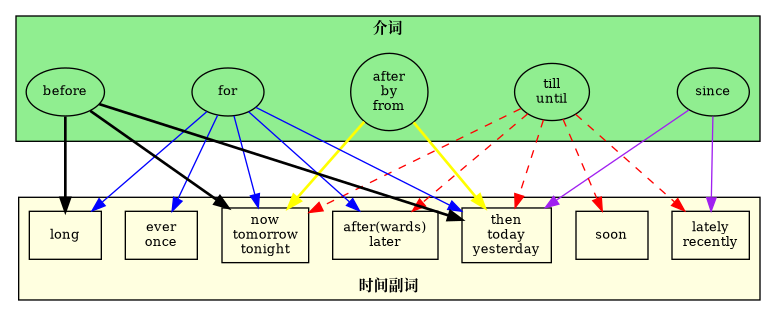
\includegraphics[width=\textwidth]{preptimeadverb.png}
  \caption{\label{fig:preptimeadv}最常用作介词补足语的时间副词}
\end{figure}


% #+BEGIN_SRC dot :file preptimeadverb.png :cmdline -Kdot -Tpng :exports results
%   digraph {
%     fontsize=11
%     fontname="serif bold"
%     rankdir="TB"
%     ranksep=0.8
%     node[shape=box fontsize=10]

%     subgraph  cluster_prep {
%       bgcolor="lightgreen"
%     rankdir="LR"
%       label=介词
%       node [shape=ellipse]
%       since
%       "B1_invis" [shape=none Xstyle=invis label="" fixedsize=true  width=0.4 height=.02]
%       till[label="till\nuntil"]
%       "B3_invis" [shape=none Xstyle=invis label="" fixedsize=true  width=0.4 height=.02]
%       afterl[label="after\nby\nfrom"]
%       "B2_invis" [shape=none Xstyle=invis label="" fixedsize=true  width=0.4 height=.02]
%       for
%       "B4_invis" [shape=none Xstyle=invis label="" fixedsize=true  width=0.4 height=.02]
%       before
%     }

%     subgraph cluster_adv {
%       bgcolor="lightyellow"
%     // rankdir="LR"
%     labelloc="b"
%       label=时间副词
%       lately[label="lately\nrecently"]
%       then[label="then\ntoday\nyesterday"]
%       now[label="now\ntomorrow\ntonight"]
%       afterr[label="after(wards)\nlater"]
%       soon
%       ever[label="ever\nonce"]
%       long
%     }


%     splines=false

%     since -> {lately, then}[color = "purple"]
%     till -> {lately,then,now,afterr,soon} [style=dashed color="red"]
%     afterl -> {then, now}[style=bold color="yellow"]
%     for -> {then, now, afterr, ever, long}[style=solid color="blue"]
%     before -> {then, now, long}[style=bold]
%   }
% #+END_SRC


\subsection{副词小品词up, down, back, away等}

down, in, up 等有时不是介词,而是副词。如以下句子中,左边介词(后接宾语),右
边为副词小品词(无宾语)。
\begin{taskitem}(2)
* I ran \unbf{down} the road.
* Please sit \unbf{down}.
* Something's climbing \unbf{up} my leg.
* She's not \unbf{up} yet.
* He's \unbf{in} his office.
* You can go \unbf{in}.
\end{taskitem}

这种短小的副词通常被叫作“副词小品词”,包括:about, above, across, ahead,
along, (a)round, aside, away, back, before, behind, below, by, down,
forward, home, in, near, off, on, out, over, past, through, under, up.

许多词既可用作副词小品词,也可用作介词,但也有例外: back, away (只能作副词小
品词); from, during (只能是介词).

副词小品词往往与动词连用,构成双词动词,有时会有全新意思(如break down, put
off, work out, give up),通常被叫做“\textbf{短语动词}”

副词小品词和形容词一样,往往用作be动词的补语。
\begin{itemize}
\item Why are all the lights \unbf{on}?
\item The match will be \unbf{over} by 4.30.
\item Hello! You're \unbf{back}!
\item I'm \unbf{off} – see you later!
\end{itemize}

\subsection{形容词和副词的比较级}

\subsubsection{可分等级的形容词和副词类型}

可分等级的形容词和副词可以有三种类型的比较,即:
\begin{description}
\item[向较高程度的比较] 通过屈折变化 -er 和 -est;迂回法 more和most的比较级、最高
  级表示(见\cref{tab:comparison})。

\item[相同程度的比较] 通过as/so \ldots{} as表示。
  \begin{itemize}
  \item Anna is \unbf{as tall as} Bill.
  \item Anna is not \unbf{as/so tall as} Bill.
  \end{itemize}

\item[向较低程度的比较] 通过little的比较级less 和最高级 least表示。
  \begin{itemize}
  \item This problem is \unbf{less difficult} than the previous one.

    这个问题比上题难度低。
  \item This is the \unbf{least difficult} problem of all.

    这是所有问题中最简单(不困难)的。
  \end{itemize}
\end{description}

\begin{table}[htbp!]
  \centering \small
  \begin{talltblr}[ caption = {形容词和副词的比较级},
    label = {tab:comparison},
    ]{
      width=\linewidth, colspec={llll},
      rowsep=2pt, colsep=4pt,
      row{1} = {font=\bfseries},
    }
    \toprule
    & 原级 & 比较级 & 最高级 \\\midrule
    \textbf{屈折变化形式} \\
    形容词 & high & higher & highest \\
    副词 & soon & sooner & soonest \\ \hline
    \textbf{迂回法形式} \\
    形容词 & complex & more complex & most complex \\
    副词 & comfortably & more comfortably & most comfortably \\
    \bottomrule
  \end{talltblr}%
\end{table}

\subsubsection{不规则的比较级、最高级形式}

不规则的比较级、最高级形式较少(见\cref{tab:composison})。

\begin{table}[htbp]
  \centering \small
  \begin{talltblr}[ caption = {不规则的比较级和最高级},
    label = {tab:composison},
    ]{
      width=\linewidth, colspec={lll},
      rowsep=2pt, colsep=4pt,
      row{1} = {c, font=\bfseries},
    }
    \toprule
    原形 & 比较级 & 最高级 \\  \midrule
    bad/sick/evil & worse & worst \\
    far(通用,进一步)& further & furthest  \\
    far (时空距离远) & farther & farthest \\
    good/well & better & best \\
    in & inner & innermost \\
    little & less & least \\
    many/much/a lot & more & most \\
    old & older/elder & oldest/eldest \\
    out & outer & outermost \\
    \bottomrule
  \end{talltblr}%
\end{table}

其中,farther/farthest 和 further /furthest 这两组词既是形容词又是副词。
farther/farthest主要只用来表达物理时空距离较远、最远。further /furthest则囊
括上述含义,并且还可以有“进一步,较多,最近” (more, additional, later) 的意思。

\begin{itemize}
\item I have to travel \unbf{further/farther} to work now.

  现在我得走更远的路去上班。

\item Let's consider this point \unbf{further}.

  让我们更深入地考虑这一点。

\item The school will be closed until \unbf{further} notice.

  学校将关闭,直至进一步的通知。
\end{itemize}

elder其实不是真正的比较级形式,因为在它后面不能跟 than,而要用规则屈折变
化older。elder只能指人,并多用在家庭成员出生顺序,如elder brother/sister表示
哥哥、姐姐。

\subsubsection{规则的比较级屈折变化}

\begin{itemize}
\item 以单个元音字母+单个辅音字母结尾的形容词,先双拼辅音字母,再加 -er和-est 。

  big \~{} bigger \~{} biggest \qquad sad \~{} sadder \~{} saddest

\item 以辅音字母 + y 结尾的形容词,先把 y 改为 i,再加 -er和-est。

  angry \~{} angrier \~{} angriest \qquad early \~{} earlier \~{} earliest

\item 词尾以哑音 -e 结尾,去掉 e,再加 -er和-est。

  pure \~{} purer \~{} purest \qquad brave \~{} braver \~{} bravest

  -ee结尾的去掉末尾的e,再加 -er和-est。

  free \~{} freer \~{} freest

\end{itemize}

\subsubsection{屈折法比较和迂回法比较之间的选择}
\begin{itemize}
\item 一般来讲,单音节形容词通常用屈折变化。

  例外是real, right, wrong 和介词 like只用迂回形式来构成比较级和最高级。

\item 大部分双音节形容词既可以用屈折变化,也可用迂回法。

  对于以 -ing, -ed, -ful, -less等类复合词的双音节形容词来说,只能用迂回法。

\item 三个及以上音节的形容词,只能用迂回法。

  带否定前缀 un- 的形容词两者都可用:
  \begin{itemize}
  \item unhappy \~{} unhappier / more unhappy \~{} unhappiest / most unhappy

  \item untidy \~{} untidier / more untidy \~{} untidiest/ most untidy
  \end{itemize}
\item 以 -ly 结尾的开放式副词可能因音节数量问题,不能用屈折变化,只能用迂回法。
\end{itemize}

\subsubsection{比较级和最高级中冠词的用法}

\begin{itemize}
\item 比较级出现在than结构中,一般不用加the。


\item 最高级 + of (all) 结构中,最高级前要加the。

\item 最高级作定语,修饰名词中心语,最高级前要加the或其他定指限定词。
  \begin{itemize}
  \item Anna is \unbf{the/their youngest} child.

  \item Della is the/our most efficient publisher. \quad efficient
    \doulos{/ɪˈfɪʃnt/} 效率高的;有功效的
  \end{itemize}

  如果形容词不是起定语作用,the 就可有可无:
  \begin{itemize}
  \item Anna is (the) youngest (of all).
  \end{itemize}
\end{itemize}

重复和并列比较级表示程度逐渐增强,不加冠词。
\begin{itemize}
\item She is getting better and better.

\item They are becoming more and more difficult.
\end{itemize}


\subsubsection{比较级的前置修饰语}

形容词和副词的原级可为强化语(如 very, quite, so 等)所前置修饰。
\begin{itemize}
\item The job was \unbf{very easy}.
\end{itemize}

形容词和副词的比较级,不论是屈折变化形式,还是迂回形式,都可由增强
语(如 much, far 或 very much) 前置修饰:
\begin{itemize}
\item The job was \unbf{(very) much/far easier(more difficult)} than I thought.
\item She writes \unbf{(very) much/far better} than she used to.
\end{itemize}

下面是常常与比较级连用的其他强化语(和强化名词短语):
\begin{itemize}
\item somewhat/rather easier than \ldots{}
\item a lot/great/good/ easier than \ldots{}
\end{itemize}

\section{状语的语义和语法}

\subsection{状语按语义分类}

状语按语义可分为以下几类(也是状语的作用)
\begin{enumerate}
\item \textbf{空间}

  \begin{description}
  \item[位置] The dog was asleep \unbf{on the grass}.
  \item[方向] They walked \unbf{down the hill}.
  \item[目标] She hurried \unbf{to the station}.
  \item[来源] This book cannot be taken \unbf{from the library}.
  \item[距离] We mustn't go \unbf{very much further}.
  \end{description}
\item \textbf{时间}

  \begin{description}
  \item[固定时间位置] She was born \unbf{in 1980}.
  \item[前跨延续] I shall be in Chicago \unbf{until Thursday}.

    以“现在时间”为基点,向前跨越。
  \item[后跨延续] We have been at the airport \unbf{since yesterday}.

    以“现在时间”为基点,向前跨越。或者说从过去某时间点到现在。

  \item[时间频度] They \unbf{very seldom} went to see their parents.
  \item [一个时间和另一个时间的关系] She must \unbf{still} be in her office.
  \end{description}

\item \textbf{方式过程}

  \begin{description}
  \item[方式] The minister explained his policy \unbf{very clearly}.
  \item[手段] \unbf{By her insight}, she grasped the patient's real problem.
  \item[工具] I have difficulty eating \unbf{with chopsticks}.
  \item[施事] Penicillin was discovered \unbf{by Sir Alexander Fleming}.
  \end{description}

\item \textbf{方面}, 用状语增加具体真实价值。
  \begin{itemize}
  \item She helped him \unbf{with his research}.

    她帮助他做研究。
  \item He's busy writing.
  \end{itemize}
\item \textbf{原因}
  \begin{description}
  \item[原因] She died \unbf{of cancer}.
  \item[理由] He bought the book \unbf{through an interest in China}.
  \item[目的] He bought the book \unbf{to study English}.
  \item[结果] He always studies hard, \unbf{so he has good grades}.
  \item[条件] \unbf{If he always studies hard}, he will have good grades.
  \item[让步] \unbf{Even though he studied hard}, he didn't have good grades.
  \end{description}

\item \textbf{情态},可以使用状语来改变句子的真实性(如增强或减弱)。
  \begin{description}
  \item[强调] She \unbf{certainly} helped him with his research.

  \item[近似] They are \unbf{probably} going to the zoo.

  \item[限制] I shall be in Chicago \unbf{only} until Thursday.
  \end{description}

\item \textbf{程度},程度状语在改变句子的真实性上与情态状语类似,但是,程度状语添加了一
  个特殊的语义成分,可分等级性。
  \begin{description}
  \item[增强语义] He \unbf{badly} needed consolation.

    他急需安慰。badly在这里是非常,很,严重的意思。

  \item[减弱语义] She helped him \unbf{a little} with his research.
  \end{description}
\end{enumerate}

\subsection{可构成状语的词类}

状语成分可以由很多词类来实现:
\begin{description}
\item[封闭类副词为中心词的副词短语] \unbf{(Just) then}, the telephone rang.
\item[以开放类副词为中心词的副词短语] You should have opened it \unbf{(a bit more) carefully}.
\item[名词短语] They had traveled \unbf{a very long way}.
\item[介词短语] Tom hurried \unbf{across the field}.
\item[无动词分句] \unbf{When in doubt} the answer is ``no''. doubt, 疑问。
\item[非限定性分句] \unct{She}{S} \unct{realized}{V}, \unct{lying there}{A}, \unct{what she must do}{O}.
\item[限定性分句] We sent for you \unbf{because you were absent yesterday}.

  我们叫你来是因为你昨天缺席了。
\end{description}

\subsection{状语的位置}

与其他句子成分相比,状语成分可以比较自由地被置于句内各个不同的位置上(简单了
解即可):
\begin{description}
\item[I] \unbf{by then} the book should have been returned to the library.
\item[iM] The book \unbf{by then} should have been returned to the library.
\item[M] The book should \unbf{by then} have been returned to the library.
\item[mM] The book should have \unbf{by then} been returned to the library.
\item[eM] The book should have been \unbf{by then} returned to the library.
\item[iE] The book should have been returned \unbf{by then} to the library.
\item[E] The book should have been returned to the library \unbf{by then}.
\end{description}

如上文中的符号所示,状语可位于句中三个主要位置:句首位置I(NITIAL),句中位
置M(EDIAL),句末位置E(ND),但是,句中位置又分有三个变体(句中首位iM,句中中
位mM和句中末位eM)以及句末位置下分的句末首位(iE)。\textbf{句中位置就是紧接在功能词
  或系词后面的位置。}

若不存在功能词,那么M的位置就简单的处于S和V 之间;若S被省略,M的位置则位于V的
前面。

状语位置的选择由语义和语法因素来决定,但是同时也由信息处理的要求和末端
重 (end weight)原则来决定。如果没有特殊因素需要考虑,状语应被置于E(句末位
置),事实上,状语多数被置于这个位置。

\subsubsection{各类状语位置}

连接状语 Connecting adverbials 和评论状语 comment adverbials多表示本句与其他
句子的关系,或者评价本句,所以通常放在句首:
\begin{itemize}
\item \unbf{However}, not everybody agreed.

\item \unbf{Fortunately}, nobody was hurt.
\end{itemize}

Adverbials of indefinite frequency, certainty and completeness

不定频度状语(always, often等),确定性状语(probably, definitely等) 和完整性状
语 (completely, almost等) 通常放在句中。
\begin{itemize}
\item My boss \unbf{often} travels to America
\item I've \unbf{definitely} decided to change my job.
\item There is \unbf{clearly} something wrong.
\item The builder said he had \unbf{almost} finished, but it wasn't true.
\item \unbf{Sometimes} I'd like to live alone somewhere else alone.
\end{itemize}

焦点状语Focusing adverbials (also, just, even等)可以放在句中或其他位置,依具
体状语而定。
\begin{itemize}
\item He's \unbf{even} been to Antarctica.

\item We are \unbf{only} going for two days.


\item \unbf{Once} you could do a thing like that.

  只有你才会做出那样的事。
\end{itemize}

Adverbials of manner (how), place (where) and time (when) most often go in end position.

方式、地点和时间状语通常放在句中:
\begin{itemize}
\item She brushed her hair \unbf{slowly}.
\item The children are playing \unbf{upstairs}.
\item I phoned Alex \unbf{this morning}.
\end{itemize}

时间状语也可以放在句首。
\begin{itemize}
\item \unbf{Tomorrow} I've got a meeting in Cardiff.
\end{itemize}

强调状语Emphasizing adverbials (terribly, really等) 通常与其所强调的词放在一
起。
\begin{itemize}
\item I'm \unbf{terribly} sorry about last night.
\end{itemize}

程度状语 Degree adverbials (more, very much, most, a lot, so等) 据其功能位置可变

如有多条状语短句,通常按照方式、地点、时间的顺序排列。
\begin{itemize}
\item Put the butter \unbf{in the fridge} \unbf{at once}. (not … at once in the fridge.)
\item Let's go \unbf{to bed} \unbf{early}. (not … early to bed.)
\item I worked \unbf{hard} \unbf{yesterday}.
\item She sang beautifully \unbf{in the town} \unbf{hall last night}.
\end{itemize}

\subsubsection{分裂不定式}
\label{subsubsec:splitinf}

\begin{description}
\item[分裂不定式 (SPLIT INFINITE)] \index{概念!分裂不定式 split infinite} \textbf{句中末位状语}用在 to 和不定式的助动词之后,
  主要动词之前。
  \begin{itemize}
  \item He wasn't able to \unbf{even} move his fingers.
  \item She ought to \unbf{seriously} consider her position.
  \item She ought to have \unbf{seriously} considered her position.

    她应该认真考虑下自己的立场。

  \item Your task is to \unbf{really} understand your students' problems.
  \item I do TR\`Y to underST\'AND --- to TR\`ULY understand.

  \item No one invited me to \unbf{so much as} have a glass of water. [甚至]

    甚至没有人请我喝杯水。
  \end{itemize}
\end{description}

分裂不定式因文体在200多年里一直受到一些指责,但另一些专家认为这是可以接受的。

to cheerfully sing in the bath
\section{介词和介词短语}

\subsection{介词补语}

介词表达两个实体之间的关系,其中一个实体以介词补足语为代表。

介词补足语通常都是名词性短语(含名词短语、代词、-ing分句、wh-名词性分句)。

介词短语本身也可以用作介词补足语,如:
\begin{itemize}
\item We didn't meet \unbf{until after the show}.

\item The weather has been fine \unbf{except in the north}.
\end{itemize}

\textbf{尽管that分句和不定式分句可以起名词作用,但是它们不能作介词补语。}\textbf{人
称主格} I, you等也不能。

\begin{itemize}
\item I was surprised $ \left\{
    \begin{aligned}
     &\text{\unbf{at} her angry response.}\\
     &\text{\unbf{at} hearing her objecti on.}\\
     &\text{\unbf{at} what she said.}\\
     &\text{to hear her objection.}\\
     &\text{that she responded so angrily. }
    \end{aligned}
  \right. $

\end{itemize}

\subsection{介词、连接词和动词}
\label{subsec:prepconn}

介词和连接词都具有关联或连接功能,试比较:
\begin{itemize}
\item The day \unbf{when} she arrived. [连接词]
\item The day \unbf{of} her arrival. [介词]
\end{itemize}

某些情况下,同一词项既可以作介词又可以作连接词,如\textbf{after, as, before, since, until}.
\begin{itemize}
\item the day$ \left\{
      \begin{aligned}
        &\text{\textbf{before} she arrived} [连接词]\\
        &\text{\textbf{before} her arrival} [介词]\\
      \end{aligned}
    \right. $
\end{itemize}

辨别这两个词类的一个标准是:介词引导的是\textbf{名词性或名词化补足语};而与之对应的连
接词(从属连词)引导的是一个\textbf{从句}。

% Please add the following required packages to your document preamble:

% \usepackage{tabularray}
% \UseTblrLibrary{booktabs}
% \UseTblrLibrary{nameref}

\begin{table}[htbp]
  \centering
  \begin{talltblr}[ caption = {介词和连接词后面的结构},
    label = {tab:prepconn},
    ]{
      width=\linewidth, colspec={cccc},
      rowsep=2pt, colsep=4pt,
      row{1} = {c, font=\bfseries},
    }
    \toprule
    后接结构 & when连接词 & after连接词或介词 & by 介词 \\ \midrule
    限定分句 & when she spoke & after she spoke & \xout{by she spoke} \\
    非限定分句 & when speaking & after speaking & by speaking \\
    名词短语 & \xout{when her speech} & after her speech & by her speech \\
    \bottomrule
  \end{talltblr}%
\end{table}

有些 -ing 和 -ed 分句形式就可以有边缘介词 (marginal preposition)、非限定动词
形式的功能,又可以有连接词的功能,如 considering 和 given.

\begin{description}
\item[分词作介词] 接名词性(化)短语
  \begin{itemize}
  \item \unbf{Considering his age}, he has made excellent progress in his studies.

    [等同于 If one considers his age \ldots 或 In view of his age \ldots{}]

  \item \unbf{Given the present conditions}, I think she's done rather well.

    [等同于 If one takes into account \ldots{}。 take into account是习
    语 idiom:考虑到、顾及到]
  \end{itemize}

\item[分词] 非限定性分句
  \begin{itemize}
  \item \unbf{Considering the conditions in the office}, she thought
  \end{itemize}

\item[连接词]
  \begin{itemize}
  \item \unbf{Considering (that) he is rather young}, his parents have advised
    him not to apply.

  \item \unbf{Given (that) the weather is expected to be sunny tomorrow}, we should
    plan a picnic.
  \end{itemize}
\end{description}

其他可作连接词的现在分词形式还有seeing (that) 和 provided (that)等(连接词表详见\cref{subsec:subcon})。


\subsection{介词后置}

\index{介词后置}
尽管介词一般在它本身补语的前面,但是,在一些情况下,介词必须后置:
\begin{itemize}
\item \textbf{介词动词}的\textbf{被动语态}结构,其中主语相当于主动语态里的介词
  补语:
  \begin{itemize}
  \item \unbf{The car} has been paid \unbf{for}.
  \end{itemize}

\item \textbf{介词补足语主位化}的不定式分句 或 -ing分句:
  \begin{itemize}
  \item \unbf{That man} is unpleasant to work \unbf{with}.

  \item \unbf{His advice} is not worth listening \unbf{to}.
  \end{itemize}

  因上,当疑问词或引导词是介词补足语时,介词往往出现在句尾,尤其是非正式用法
  中。
  \begin{itemize}
  \item \unbf{What} are you looking \unbf{for}?
  \item \unbf{Who} is she talking \unbf{about}?
  \item \unbf{About whom} is she talking? 太正式,日常不大用。
  \item \unbf{What} kind of films are you interested \unbf{in}?
  \item Tell me \unbf{what} you're worried \unbf{about}.
  \end{itemize}

  可是,当名词与疑问词连用一体时,介词不后置。
  \begin{itemize}
  \item \unbf{With} what money? (不能说 \sout{What money with.})
  \end{itemize}

\item 一些简单介词(如through)和多数的复杂介词(如because of, in addition
  to)不可以被后置。

\end{itemize}

\subsection{简单介词和复杂介词}

最普通的介词是一些单音节词项,如 at, for, in, on, to, with,\textbf{除非被后
  置},它们通常要\textbf{非重读且元音弱化}。

有一些多音节介词,它们中有的向来就是由单音节介词组成的复合词(例如: inside,
with in),有的源于分词(例如: during, concerning, granted),有的由其他语言引
入(例如: despite, except)。

介词数量的增加主要是由于介词与其他词组成了“\textbf{复合介词}”。复合介词主要
有两大类:
\begin{description}
\item[分词、形容词、副词、或连词 + 简单介词] 如:owing to, devoid of, away
  from, because of \ldots{}
\item[介词1 + 名词 + 介词2] 如:in charge of, by means of, at variance with,
  in addition to, as a result of \ldots{}
\end{description}

\subsection{表示空间关系的介词}

\begin{figure}[tp!]
  \centering
  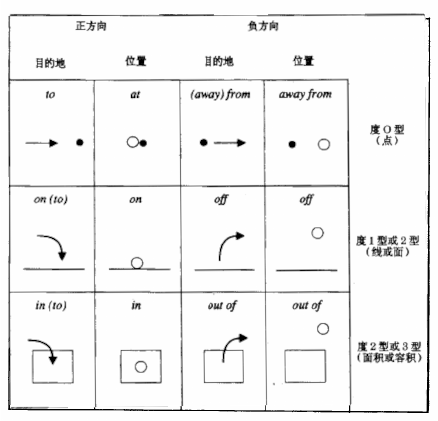
\includegraphics[width=0.8\textwidth]{prep1.png}
  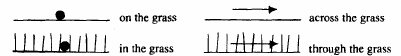
\includegraphics{prep2.png}
  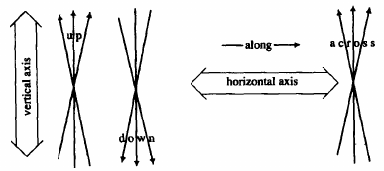
\includegraphics{prep3.png}
  \caption{\label{fig:preppic}表示空间关系的部分介词}
\end{figure}

\begin{description}
\item[over, under] 垂直关系,或者空间上接近。

\item[above, below] 仅表示“高于(低于)……水平上”

\item[among, between] among是在非分离的物体之中;between是在两独立物体之间:
  \begin{itemize}
  \item The house stands$ \left\{
      \begin{aligned}
        &\text{\emph{between} two farms.} \\
        &\text{\emph{among} farms.}
      \end{aligned}
    \right. $

  \item He likes getting \emph{among} people. [likes mixing with]
  \end{itemize}

\end{description}

其他略。

\subsection{表示时间的介词}

时间范围内一般只有两种度型,\textbf{时间点}和\textbf{时间段}。

\begin{description}
\item[时间位置 at, on, in, by]
  \begin{description}

  \item[at] 时间点和节假日
    \begin{itemize}
    \item at 6:30 pm, at the weekend, at noon, at Christmas

    \item 有些时间段被当作时间点来考虑,如:

      at night, at the/that time, at breakfast time
    \end{itemize}

  \item[on] 当作时间段看待的一天
    \begin{itemize}
    \item on Monday, on New Year's Day


    \item 时间有补足语时

      on the following day, on Monday morning, on Saturday afternoon, on the
      morning of 1 June

      但当补足语为early时,用in

      in the early morning, in the late afternoon
    \end{itemize}

  \item[in, during] 比一天更长或更短的时间段
    \begin{itemize}
    \item in the 18th century, in 1980, in August, in summer, in the evening

    \item during the 1990s, during Holy Week, during the night (during the = by)
    \end{itemize}
  \end{description}

\item[过去或将来时间段]
  \begin{description}
  \item[后置副词ago] 过去某一时间点之前的时间段

    \begin{itemize}
    \item We met \unbf{three months ago}.
    \end{itemize}

  \item[将来 in] 从现在起到未来之间的时间段
    \begin{itemize}
    \item We'll meet$ \left\{
        \begin{aligned}
          &\text{\emph{in three months' time}.} \\
          &\text{\emph{(in) three months from now}.} \\
        \end{aligned}
      \right. $
    \end{itemize}
  \end{description}

\item[持续时间段 for, during, over, (all) through, throughout]
  \begin{description}
  \item [for 持续整个时间段] for the summer

  \item[during 时间段中的某个时间段] during the (whole/stay) meeting

    如在during之后加whole/stay 修饰的话,则表示整个时间段。


  \item[over, through(out)] over通常和表示特殊日子的名词短语搭配,因
    此所指的时间一般比 through(out) 所指的更短。
    \begin{itemize}

    \item over the holiday/weekend/Sabbath, over holiday/night

    \item through(out) the summer
    \end{itemize}

  \end{description}
\item[before, after, since, till, until] 既是介词,有时连接词。

  作介词时,后面接:
  \begin{description}
  \item[时间名词短语] after next week
  \item[无主语 -ing 分句] since leaving school
  \item[从动词派生的或相当于分句的名词短语] till/until the fall of Rome,
    before the meeting
  \end{description}

\item[between \ldots{} and, by]
  \begin{description}
  \item[between \ldots{} and] 也表示时间段中的一个小时间段,还可以表示重复出
    现的相同事物之间的间隔。
    \begin{itemize}
    \item between 5 and 6 o'clock, between lunch and dinner

    \item  between meals/dances/acts/classes
    \end{itemize}

  \item[by] 事件结果出现的瞬间或时间终点。
    \begin{itemize}
    \item She should be back \unbf{by now}.

    \item \unbf{By the time} we'd walked five miles.
    \end{itemize}

  \end{description}
\item[不加时间介词的情况]
  \begin{description}
  \item[指示词last, next, this, that, some, every]
    \begin{itemize}
    \item last Thursday, next time, every month, this morning
    \end{itemize}

  \item[暗含 last, next, this指示意义的名词]
    \begin{itemize}
    \item today, yesterday, all (the) week
    \end{itemize}


  \item[时间介词可省略]
    \begin{itemize}
    \item (for) three months, (for) the whole time

    \item (on) the day before yesterday, (on) the next day
    \end{itemize}
  \end{description}
\end{description}



\subsection{表示原因和目的的介词}

\begin{description}
\item[原因、理由和动机 because of, on account of, for, out of]
  \begin{itemize}
  \item He lost his job \unbf{because of} his laziness.
  \item She was fined \unbf{for} dangerous driving .
  \item They died \unbf{from} exposure.
  \end{itemize}
\item[目的、目标和对象 for, to, at]
  \begin{description}

  \item[for]
    \begin{itemize}
    \item We had better set out \unbf{for} home.

    \item for money/love/shelter

    \item She made a beautiful \unbf{for her daughter}. [预计接收者]
    \end{itemize}

  \item[to] 实际接收者
    \begin{itemize}
    \item She gave a beautiful \unbf{to her daughter}.
    \end{itemize}

  \item[at] 暗示“希望达到某种目的”或有“敌意”
    \begin{itemize}
    \item kick/charge/bite/catch/shoot/chew at [目的不一定最终达成]
    \end{itemize}
  \end{description}
\end{description}

\subsection{表示由手段到刺激因素的介词}

介词还可以表示\textbf{手段}、\textbf{工具}用来回答 ``How?'' 问句,其中 by 可以表达使用的手
段, with 可以表达使用的工具,例如:
\begin{itemize}
\item I go to work \unbf{by} car.
\item The thief entered \unbf{by} the back door.
\item She won the match \unbf{with} her speed.
\item He managed to open the car \unbf{without} a key.
\end{itemize}

与手段和工具相反的是\textbf{施事者},施事者为\textbf{生物名词},可以引发某事。它可以用
介词 by 来表达。
\begin{itemize}
\item This picture was painted \unbf{by} Degas.

\item I was bitten \unbf{by} a neighbour's dog.
\end{itemize}

刺激和反应主要是用 at, with, about, in, of 和 to 来表达:
\begin{itemize}
\item I'm surprised \unbf{at/with} her attitude.

\item They were all angry \unbf{at/with} Tom for making such a stupid mistake.

\end{itemize}

\subsection{表示……的介词}

可以使用 from 或 out of表示\unbf{来源}(与目的相反):
\begin{itemize}
\item I don't like to borrow \unbf{from} friends.

\item She let him \unbf{out of} the house.
\end{itemize}

当 as 是“作为某个角色”的意思时,后面出现的短语表明了原因。
\begin{itemize}
\item \unbf{As} a doctor, I ought to help you.
\end{itemize}

其他略。

\subsection{介词副词}

有些介词还可以用作副词,常常像其省略了补足语的介词形式。

% Please add the following required packages to your document preamble:

% \usepackage{tabularray}
% \UseTblrLibrary{booktabs}
% \UseTblrLibrary{nameref}

\begin{table}[htbp!]
  \centering \small
  \begin{talltblr}[ caption = {可用作副词的介词},
    label = {tab:advprep},
    ]{
      width=\linewidth, colspec={lllll},
      rowsep=4pt, colsep=10pt,
    }
    \toprule
    aboard  & about   & above     & across    & after        \\
    ahead   & along   & alongside & around    & away         \\
    back    & before  & behind    & below     & beneath      \\
    besides & between & beyond    & by        & close        \\
    down    & east    & in(side)  & instead   & near         \\
    off     & on      & opposite  & out(side) & over(head)   \\
    past    & round   & since     & together  & through(out) \\
     up     & within  & without   & \SetCell[c=2]{l} under(neath)             \\
      \SetCell[c=3]{l} 复杂介词 in/on + 名词 \sout{+ 介词}        \\
    \bottomrule
  \end{talltblr}%
\end{table}

\begin{itemize}
\item A car drove$ \left\{
    \begin{aligned}
      &\text{past the door. [past 介词]} \\
      &\text{past}  [past 副词]
    \end{aligned}
  \right. $

\item Why didn't you come $ \left\{
    \begin{aligned}
	    &\text{before 7 o'clock? [before 介词]} \\
      &\text{before? [before 副词]}
    \end{aligned}
    \right. $

  \item Paul wants to go to the Zoo $ \left\{
      \begin{aligned}
        &\text{instead of staying home.} \\
        &\text{instead.}
      \end{aligned}
  \right. $
\end{itemize}

\section{简单句}

\subsection{简单句和多重句}

\begin{description}
	\item[简单句 (SIMPLE)] 只有一个\textbf{独立分句}构成的句子。\index{概念!简单句 simple sentences}

\item[多重句 (MULTIPILE SENTENCES)] 有一个及以上分句作为句子的直接成分。还可以细分为:
  \index{概念!多重句 multiple sentences}
  \begin{description}
  \item[复合句 (COMPLEX)] \index{概念!复合句 complex} \textbf{从属分句}
    (SUBORDINATE CLASUSES) 作为一个(以上)句子成分,如直接宾语或状语;通常由
    一个从属连接词 (CONJUNCTION) 引导。

  \item[联合句 (COMPOUND)] 两个或两个以上\textbf{并列}分句 (COORDINATE
    clauses)。 \index{概念!联合句 compound}


    语法等级体系中相等地位的两个或两个以上的单位,可构成一个与之性质相同的单位。
    这种结构称为\textbf{并列关系} (COORDINATION), 而且像从属关系一样,由一个称
    为连词的连接词明确表示出来.这种连词叫\textbf{并列 (COORDINATING) 连词}。
  \end{description}
\end{description}

\improve[inline]{夸克的分句分类方法与其他一些语法书不同,比较复杂,暂且不论。}

关于分句结构和成分划分可以有一种以上的分析方法。因英语中遍布各处的递差造成较
多模糊性;通常这些模糊之处并不重要,只是需要建立自己较为自洽的分析方法。

例如:如对所有的介词短语来说,附加状语或补语的界限并不清楚。
\begin{itemize}
\item They were \unbf{out of breath}. \qquad  They were \unbf{breathless}.
\item She is/feels \unbf{in good health}. \qquad  She is/feels \unbf{healthy}.

\item She is \unbf{young} and \unbf{in good health}.
\end{itemize}

和本书不同,“简单句”这一术语在其他语法书中经常用来指一个不包含另一分句的独
立分句,而不管所包含的分句是不是句子的直接成分。有些语法书,把非限定结构(这
种结构含有一个非限定动词作为动词成分)看作是短语而不是分句。我们则把这种结构
看作是分句,因为可以把它分解为分句成分。非限定分句本身就是从属性质的,因此不
能成为典型的简单句形式

\subsection{主语--谓语一致}

在英语中,最重要的一致关系类型是主语和谓语动词之间第三人称数的一致。单
数主语需要用单数动词,复数主语需要复数动词。

注意:在名词短语表示主语时,\textbf{由名词短语的中心词来决定名词短语的单复数}:
\begin{itemize}
\item \unbf{The change} in husbands' attitudes is most obvious in their families.
\item \unbf{The changes} in husbands' attitude are most obvious in their families.
\end{itemize}

分句、介词短语和副词作为主语一般算作单数:
\begin{itemize}
\item \unbf{Smoking cigarettes} \unbf{is} dangerous to your health .

\item \unbf{In the evenings} \unbf{is} best for me.
\end{itemize}

名字、标题、引文即使是复数名词短语,也算作单数。

\textbf{就近原则} (proximity) 是指\textbf{动词形式与紧靠在他前面的名词短语相
  一致}。如 either \ldots{} or \ldots{}, neither \ldots{} nor \ldots{}.
\begin{itemize}
\item Either your brakes \unbf{or your eyesight} \unbf{is} at fault.
\item Neither you, nor I, \unbf{nor anyone else} \unbf{knows} the answer.
\end{itemize}

在中国英语教学中,there be \ldots{} 也采用就近原则,但这其实是过时或者不准确
的,注意随机应变吧。
\begin{itemize}
\item There \unbf{is/are} an apple, two pears and some oranges on the table.
\end{itemize}

\subsection{否定}

\subsubsection{否定的三种类型}
\begin{description}
\item[分句否定 (CLAUSE NEGATION)] 从句法上将整个分句作为否定处理。

\item[局部否定 (LOCAL NEGATION)] 否定分句中某个成分。

\item[谓体否定 (PREDICATION NEGATION)] 一般指示用于某些助动词后面较次要的否
  定类型,否定主要动词及之后的部分(谓体)。
\end{description}

\subsubsection{分句否定}

\begin{description}
\item[动词否定] 最常见的形式。如无助动词,谓语部分加入假位 (dummy) 助动词be;
  在第一个助动词后加入否定词not。

\item[形式和意义上的否定] 使用no, not, never, none等否定一个分句成分,通过此
  方式来否定分句。

  正式文体中,否定整个分句的成分可以从它通常的位置移到句首。在这种情况下,主
  语和功能词常常需要倒装(见\cref{subsec:inversion})。


\item[意义否定但形式不否定的词] 如few, little, hardly, barely, scarely,
  rarely, seldom等词,也可实现分句否定:例如后面跟着非断定形式;或和肯定附加
  疑问句连用:
  \begin{itemize}
  \item I \unbf{seldom} get \unbf{any} sleep.

  \item \unbf{Hardly anyone} wants the job.

  \item They \unbf{scarcely} seem to care, \unbf{do they}?

  \item They \unbf{hardly} have any friends, \unbf{do they}?
  \end{itemize}

  当这些副词在文学和演说题材中作为状语或作为状语中的修饰语置于句首时,通常主
  语和功能词倒装:
  \begin{itemize}
  \item \unbf{Little did I} expect such kindness from so many.

  \item Rarely does crime pay so well as many people think.
  \end{itemize}
\end{description}

动词否定(左)和形式意义否定(右)的例句:
\begin{taskitem}(2)
  * That was \unbf{not} an accident.
  * That was \unbf{no} an accident.
  * He is \unbf{not} a friend of yours.
  * He is \unbf{no} friend of yours.
  * An honest man would \unbf{not} lie.
  * \unbf{No} honest man would lie.
  * She is\unbf{n't} a fool.
  * She is \unbf{no} a fool.
  * They are \unbf{not} staying with us \unbf{any} longer.
  * They are \unbf{no longer} staying with us.
  * I wo\unbf{n't} make that mistake ever again.
  * I will \unbf{never} make that mistake ever again.
\end{taskitem}

分句否定的一些特点:
\begin{description}
\item[否定分句后面附加补充分句]
  \begin{itemize}
  \item I haven't finished, \unbf{nor}/\unbf{and neither} have you. [附加否定
    分句]

    I've finished and \unbf{so} have you. [前后均肯定分句]

  \item I haven't finished, but Y\'OU H\`AVE. [附加肯定分句]

    I've finished, and \'YOU have T\`OO. [前后均肯定分句]
  \end{itemize}

\item[否定分句后跟赞同否定]
  \begin{itemize}
  \item ``He doesn't know Russian.'' ``N\`O, he D\`OESn't.''

  [比较: ``He knows Russian.'' ``Y\`ES, he D\`OES'']
  \end{itemize}

\item[either 和 too]
  \begin{itemize}
  \item She won't notice \unbf{any} change in you, \unbf{either}.

  [比较:She will notice \unbf{some} change in you, \unbf{too}.]
  \end{itemize}
\end{description}

\subsubsection{局部否定}

局部否定否定一个词或短语,而不否定分句。
\begin{itemize}
\item I visit them \unbf{not very often}.

\item \unbf{Not surprisingly}, they missed the train.

\item They live \unbf{not far} from us.

\item Our house has one wall with \unbf{no windows}.
\end{itemize}

\subsubsection{谓体否定}

情态助动词后停顿,强调not,用来否定谓体,而不是整个分句。

\begin{itemize}
\item They may / \unbf{'not go swimming}.

  [They are allowed not to go swimming.]

\item You can simply / \unbf{'not obey the order}.

\item She didn't / \unbf{'not like} them.
\end{itemize}

\subsubsection{否定的范围}

即使在分句否定中,否定成分以前的状语也通常不包括在否定范围之内。如:
\begin{itemize}
\item She definitely \unbf{didn't speak to him}.

  [她肯定没有跟他说话。]
\item She \unbf{didn't definitely speak to him}.

  [她不一定跟他说过话。]

\item I \unbf{wasn't L\v Istening} all the T\`IME.

  [我一直没有听。] 通过语调变化表明否定范围。

\item I \unbf{wasn't listening all the T\v IME}.

  [我不是一直在听。] 通过语调变化表明否定范围。

\item I \unbf{didn't listen} to \emph{some} of the speakers.

  我没有听一些人讲话,但听了另一些人讲话。
\item I \unbf{didn't listen to \emph{any} of the speakers}.

  我没有听任何人讲话。

\end{itemize}

\subsubsection{否定的焦点}

英语语音中用于比较或突出重点信息的\textbf{重音焦点}可以表明否定和肯定的部分。
\begin{enumerate}
\item I \unbf{didn't take John to swim in the P\`OOL today}.

  [didn't do so]
\item I \unbf{didn't take J\v OHN} to swim in the pool today.

  [it maybe Mary]
\item I \unbf{didn't take John to SW\v IM} in the pool today.

  [just go to the pool, but they don't swim ]
\item I \unbf{didn't take John to swim in the P\v OOL} today.

  [may take John to the seaside]
\item I \unbf{didn't take John to swim in the pool toD\v AY}.

  [maybe yesterday]
\item \unbf{\v I didn't} take John to swim in the pool today.

  [someone else takes John to do so]
\end{enumerate}

还可以:
\begin{itemize}
\item I \unbf{didn't leave H\v OME} because I was afraid of my \unbf{F\`Ather}.
\item I \unbf{didn't leave home because I was afraid of my F\v Ather}.

  [I had left home, but it wasn't because of my father.]
\end{itemize}

\section{句子类型和话语功能}

简单句可以分为四种主要句法类型,并与话语功能息息相关。
\begin{description}
\item[陈述句] 句子有主语,并且主语位于动词前:
  \begin{itemize}
  \item \unbf{Richard} \unbf{gave} Tom a watch for his birthday.
  \end{itemize}

  另外,一些句子因情景中已暗含主语,省略了主语
  \begin{itemize}
  \item (I'm) Sorry I couldn't be there.

  \item (It's) Good to see you.
  \item (I'll) See you later.
  \end{itemize}

  另外 there/here be 陈述句中,主语在谓语 be 动词之后。这其实是存在句,
  见 \cref{subsec:behave}。

\item [疑问句] 一般分为如下两种:
  \begin{description}
  \item [一般 (yes-no) 疑问句] 如果没有助动词,则加一个假位助动词DO,如例句中
    的did;且将句子中的\textbf{第一助动词}前置于主语之前,:
    \begin{itemize}
    \item \unbf{Did} \unbf{Richard} \unbf{gave} Tom a watch for his birthday?

      疑问句通常在信息中心上用升调。上句可将升调放在watch或birthday,两者有着
      不一样的焦点。
    \end{itemize}

  \item [特殊 (Wh-) 疑问句] wh- 特殊疑问词位于句首,后接一般疑问句样式:
    \begin{itemize}
    \item \unbf{What} \unbf{did} \unbf{Richard} give Tom for his birthday?
    \end{itemize}
  \end{description}

\item[祈使句] 一般没有明显的主语,并且使用动词原形:
  \begin{itemize}
  \item \unbf{Give} Tom a watch for his birthday.

  \item \unbf{Let us all} \unbf{work} hard.

    宾格主语前加let,宾格后加动词原形。
  \end{itemize}


\item[感叹句] 句子由在名词短语中作\textbf{前位限定词的 what}, 或作\textbf{形
    容词、副词或分句强化语的 how} 及相关语句成分(如\textbf{宾语、补语、状语
    和主语})前置引导。

  wh- 成分可以是:
  \begin{description}

  \item[主语] \unbf{What a beautiful girl} came!
  \item[宾语] \unbf{What a fine watch} he received for his birthday!

  \item[补语] \unbf{How beautiful} she is!

  \item[状语] \unbf{How quickly} you eat!

    \unbf{What a long time} we've been waiting!

  \item[介词补足语] \unbf{What a mess} the room was in!
  \end{description}
\end{description}

\subsection{Wh- 疑问句}

Wh- 疑问句是由简单的疑问词协助构成的 (或 wh- 词),如: who/ whom/whose,
what, which, when, where, how, why。

\textbf{不同于 yes-no 疑问句的是,Wh-疑问句一般是降调。}

\textbf{带有 wh- 词的介词性补语}:
\begin{description}
\item[正式体]介词 + wh- 位于句首
  \begin{itemize}
  \item \unbf{To whom} should I write?
  \item \unbf{In which} city did you grow up?
  \item \unbf{At what} time does the train depart?
  \end{itemize}
\item[非正式体] wh- 位于句首
  \begin{itemize}
  \item \unbf{Whom} should I write \unbf{to}?
  \item \unbf{Which} city did you grow up \unbf{in}?
  \item \unbf{What} time does the train depart \unbf{(at)}?
  \end{itemize}

\item[工具、原因和目的] 就表示工具,原因,和目的的附加成分发问,wh- 位于句
  首
  \begin{itemize}
  \item \unbf{What} shall I mend it with?
  \item \unbf{What} are you fighting for?
  \end{itemize}
\end{description}

\subsection{其他疑问句}
\begin{description}
\item[否定的一般疑问句] 否定的疑问句,倾向于否定,但像一般疑问句一样回答。如:
  \begin{itemize}
  \item \unbf{Didn't} you believe me?

  \item \unbf{Aren't} you joining us this evening?

  \item \unbf{Haven't} he told you what to do?

  \item \unbf{Have} they \unbf{never} intited you home?
  \end{itemize}
\item[附加疑问句] 前半句为肯定或否定陈述句,后半句一般是相反的疑问。如:
  \begin{itemize}
  \item The boad \unbf{hasn't} left, \unbf{has} it?
  \item She \unbf{knows} you, \unbf{doesn't} she?
  \end{itemize}

  附加疑问句的核心语调落在助动词上,升调或降调表示不同倾向。夸克用 + 表示肯
  定,- 表示否定,如下:
  \begin{description}
  \item[+\`S -\'T] 附加疑问是升调,表倾向中性。如:
    \begin{itemize}
    \item He \unbf{likes} his J\`OB, \unbf{D\'OESn't} he?
    \end{itemize}
  \item[-\`S +\'T] 附加疑问是升调,表倾向中性。如:
    \begin{itemize}
    \item He \unbf{D\`OESn't} likes his J\`OB, \unbf{DOES} he?
    \end{itemize}
  \item[+\`S -\`T]
    \begin{itemize} 附加疑问是降调,倾向与陈述句一样。如:
    \item He \unbf{likes} his J\`OB, \unbf{D\'OESn`t} he? [肯定倾向]
    \end{itemize}
  \item[+\`S -\`T] 附加疑问是降调,倾向与陈述句一样。如:
    \begin{itemize}
    \item He \unbf{doesn't} like his J\`OB, \unbf{D\`OES} he? [否定倾向]
    \end{itemize}

  \item[+\`S + \'T] 比较少见的句式是陈述部分和附加疑问都是肯定,常有训斥或讽刺意味。如:
    \begin{itemize}
    \item Oh, you\unbf{'ve} had another \`ACcident, \unbf{H\'AVE} you?
    \item So that\unbf{'s} your G\`AME, \unbf{\'IS} it?
    \end{itemize}
  \end{description}


\item[回响疑问句] 重复部分或者是全部已讲过的话,以期得到确认。
\begin{itemize}
\item A: The Browns are emigrating. \qquad B: \unbf{\'Emigrating?}
\item A: He's a doctor. \qquad B: \unbf{Wh\'at} is he?
\item A: I'll pay for it. \qquad B: You'll \unbf{wh\'at}?
\item A: Have you ever been to BJ? \qquad B: Have I ever been \unbf{wh\'ere}?
\end{itemize}

\item[陈述疑问句] 随便文体,多用于口语;形式上和陈述句一致,句尾语调是疑问句
  的升调;希望得到听话人的认可。如:
  \begin{itemize}
  \item You've got a \unbf{D\'OCtor}?
  \item He didn't finish the \unbf{R\'ACE}?
  \end{itemize}
\end{description}


\section{替代形式和省略}

\subsection{替代形式}

\subsubsection{the same}

\begin{itemize}
\item A: Can I have \unbf{a cup of tea}, please?

  B: Give me \unbf{the same}, please.

\item Yesterday I felt \unbf{sad} and today I feel \unbf{the same}.

\item The Denison house is \unbf{small but very comfortable}, and ours is
  just \unbf{the same}.

\end{itemize}

\subsubsection{one, ones, some}

有两种替代形式的 one :一种复数形式是 some;另一种复数形式是ones。两种
都是\textbf{非重音}(因此与数字 one 区分),而且都替代\textbf{可数名词}。

some 也可以替代\textbf{不可数名词}。
\begin{itemize}
\item Have you any \unbf{knives}? I need a sharp \unbf{one}.
\item I like those \unbf{shoes}, but let's buy these \unbf{ones}.

\item Shall I pass \unbf{the butter}? Or have you got \unbf{some} already?
\end{itemize}


\subsubsection{so}
\begin{itemize}
\item You asked me to leave, and 'so I  \textbf{\textsc{d\`id}} .
\item You asked me to leave, and  I \textbf{\textsc{d\`id so}}.
\item A: It's starting to snow. B: 'So it \textbf{\textsc{\`is}} !
\end{itemize}

\subsection{省略}

\subsubsection{省略是省约的一种}

\textbf{省略} (ellipsis) 可以严格地被称为\textbf{语法省约} (grammatical omission),它有别于语
言中其他省约类型,譬如单词的\textbf{词首音节脱落} (apheresis) (cos = because , 'k
you = thank you,'d you = would you rather),\textbf{单词的截短法} (influenza = flu)
和\textbf{语义蕴含} (Frankly, \ldots{} )等。

省略与其他省约类型的区别主要在于,省略强调:
\begin{description}
\item[逐字还原 (VERBATIM RECOVERABILITY)] 能够精确恢复和重新某一段文字、发音
  和记录的内容。
\end{description}

但实际上,省略与其他省约方式仍有递差,其严格程度也有差别,并不存在完全分界线。

% Please add the following required packages to your document preamble:

% \usepackage{tabularray}
% \UseTblrLibrary{booktabs}
% \UseTblrLibrary{nameref}

\begin{table}[htbp!]
  \centering \small
  \begin{talltblr}[ caption = {省略标准的递差——从省略到其他省约},
    label = {tab:ellipsis},
    ]{
      width=\linewidth, colspec={cccccXl},
      rowsep=2pt, colsep=4pt,
      row{1} = {c, font=\bfseries},
    }
    \toprule a & b & c & d & e & 例句 & 省略类型\\ \midrule
    + & + & + & + & + & I'm happy if you are (happy). & 严格省略\\
    + & + & + & + & - & She sings better than I can (sing). & 标准省略\\
    + & ? & - & + & $\oplus$ & She works harder than him (*works). & 准省略\\
    + & + & + & - &  & (I am) Glad to see you. & 实境省略\\
    - & + & + & + & - & (Since he was / Being) Angry, he stalked out. & 弱省
    略\\
    + & ? & + & - &  & I believe (that) you are wrong. & 结构省略 \\
    - & + & + & - &  & The man (that/who/whom) I saw was half asleep. & 弱省
    略 \\
    - & ? & + & - &  & Houses (that/which are) owned by Mr Smith. & 弱省略 \\
    - & - & + & - &  & The door opened and (then/after that/\ldots{}) Mary
    entered. & 语义蕴含 \\ \bottomrule
    \SetCell[c=6]{l} \textbf{省略标准} \\
    \SetCell[c=6]{l} a: 省略词语可以准确还原。 \\
    \SetCell[c=6]{l} b: 省略的结构为语法“缺陷”。 \\
    \SetCell[c=6]{l} c: 还原词语后句子符合语法,且与原句意相同。 \\
    \SetCell[c=6]{l} d: 省略词语可根据篇章(而不是结构或实境)还原。 \\
    \SetCell[c=6]{l} e: 省略词语与先行词完全相同。\\ \bottomrule
    \SetCell[c=6]{l} \textbf{符号说明} \\
    \SetCell[c=5]{l} + \hspace{1em}符合标准 &&&&& $\oplus$ \hspace{1em} 适用
    标准须作语法变化 \hspace{2em} - \hspace{1em} 不符标准\\
    \SetCell[c=5]{l} ? \hspace{1em} 不确定  &&&&&  空白 \hspace{1em} 不涉及\\
    \bottomrule
  \end{talltblr}%
\end{table}

\subsubsection{省略的位置分类}

\begin{description}
\item[句首省略] (I) hope he's there.
\item[句中省略] Jill owns a Volvo and Fred (owns) a BMW.
\item[句尾省略] I know that we haven't studied hard yet, but we will (study hard).
\end{description}

\subsection{省略的还原类型}

\subsubsection{实境省略}

典型的实境省略是句首省略,尤其是采取\textbf{省略主语、功能词或两者都省略}这两个成
分的形式。

陈述句中的省略:
\begin{itemize}
\item (I) Told you so.
\item (I'm) Sorry I couldn't be there.
\item (It's) Good to see you.
\item (I'll) See you later.
\end{itemize}

疑问句中的省略:
\begin{itemize}
\item (Are you) In trouble?
\item (Is there) Anybody in?
\item (Do you) Want some?
\item (Have you) Got any money?
\item (Does) 'Anybody need a lift?
\item (Has) 'Jack done her homework?
\end{itemize}

\subsubsection{结构省略}

\begin{itemize}
\item I believe (that) you are mistaken.
\item We're staying there (for) another three weeks. [非正式]
\end{itemize}
\subsubsection{篇章省略}


\section{并列}
\subsection{并列连词 and, or, but}

略。

\subsection{关联连词 both \ldots{} and, either \ldots{} or, neither \ldots{}
  nor}

if \ldots{} then, whether \ldots{} or 等\textbf{关联从属连词},暂且不表。

\begin{description}
\item[either \ldots{} or] 强调 or 的\textbf{排他} (EXCLUSIVE) 含义。
  \begin{itemize}
  \item \unbf{Either} the room is too small \unbf{or} the piano is too large.

  \item \unbf{Either} Sylvia \unbf{or} her sister will be staying with us.
  \end{itemize}

\item[both \ldots{} and] 强调 and 的补充 (ADDITIVE) 含义,前后并列同等。
  \begin{itemize}
  \item Mary \unbf{both} washed the dishes \unbf{and} dried them.

  \item \unbf{Both} Mary \unbf{and} Peter washed the dishes.
  \end{itemize}

\item[nor, neither] nor或 neither 可单独用作\textbf{否定补充副词},而不是作为一对关联
  连词。他们一般预先前文明示或暗示否定意义。
  \begin{itemize}
  \item She doesn't like them and \unbf{nor} does her brother.

  \item ``I'm not going.'' ``\unbf{Nor} am I.''
  \item They never forgave him for the insult, and/but \unbf{neither/nor} could he rid
    himself of the feelings of guilt for having spoken in that way.
  \end{itemize}


\item[关联连词 neither \ldots{} nor]
  \begin{itemize}
  \item David \unbf{neither} loves Joan, \unbf{nor} wants to marry her.

  \item \unbf{Neither} peter \unbf{nor} his wife wanted the responsibility.
  \end{itemize}


\item[not (only) \ldots{} but] 不但 \ldots{} 而且
  \begin{itemize}
  \item Columbus \unbf{not only} plays hard \unbf{but also} works hard.

  \item Not only did they break in to Mr. Zhang's office, but they also stole his books.

    为加强语气,可将Not only倒装于句首,后接表强调的助动词DO + 主谓分句。

    因为传统语法认为\textbf{并列分句彼此要功能和地位相等},所以Not only倒装时,
    前后都是完整句子 they \ldots{}
  \end{itemize}
\end{description}

\subsection{准并列连词}
\label{subsec:quasicoor}

\begin{description}
\item[准并列连词 (QUASI-COORDINATORS)] \index{概念!准并列连
    词quasi-coordinators} 有时候像\textbf{并列连词},有时候又像\textbf{从属连词}或\textbf{介词}。他们有:
  \begin{description}
  \item[比较形式] as well as, as much as, rather than, more than

  \item[关联连词] not so much \ldots{} as
  \item[其他] if not, not to say
  \end{description}
\end{description}

少见,略。

\section{复合句}

\subsection{从属分句和母句}

\textbf{复合句}像简单句,因为它\textbf{只包含一个主要分句};但是和简单句不一样
的是,它\textbf{有一个或一个以上的从属分句作为它的句子成分。}

\textbf{从属和并列}相互结合可使句子更加复杂,结构更加多变。复合句的每一个主要
分句可能包含一个或多个从属分句,而每个从属分句有可能包含自己的从属分句。

\begin{itemize}
\item Although I admire her reasoning, \unbf{I reject her conclusion}.
\end{itemize}

夸克使用\textbf{母句} (MATRIX clause)来称呼去除了从属分句的领句。

分句的三种主要类型见 \cref{subsec:iffinite}。

\subsection{从属连词}
\label{subsec:subcon}

\todo[inline]{根据夸克大全14.11续写}

\subsection{非限定性分句省略方法}


由于\textbf{非限定性动词分句}(谓词为分词、不定式的句子,
见 \cref{subsec:iffinite})没有时态标记和情态助动词,又常常没有主语和从属连词;
也可以\textbf{根据句子的语境来还原时态、语态、人称和数},因此是一种很有价值
的\textbf{压缩句子}的方法。

\begin{itemize}
\item \unbf{When} (\emph{she was}) \unbf{questioned}, she denied being a member of the group.
\item (\emph{Since/Because/As they were}) \unbf{Considered works of art}, they were
  admitted into the country without customs duties.

  它们被视为艺术品,被准许免关税进入该国。
\end{itemize}

在上下文中找不到与名词性成分指称的联系时,那么主语可能是\textbf{不确定主语}或
是\textbf{说话者}。
\begin{itemize}
\item \unbf{To be an administrator} is to have the worst job in the
  world. [\emph{(For) a person}]
\item It's hard work \unbf{to be a student}. [不确定主语,根据上下文而定,
  如: (for) anyone]
\item It's hard work \unbf{to be honest}. [不确定主语,根据上下文而定]
\end{itemize}

助动词 have 有时用在 to 不定式中 (to have happened) 或 -ing 分词
中(having happened),前者更能表示未来时间或不确定性。

\subsection{无动词分句省略方法}

SVC, SVA 两种句型中,其中V为系动词且无实际意义,因此常常可以\textbf{省去系动词V},
成为\textbf{无动词分句}。

\begin{itemize}
\item Seventy-three people have drowned in the area, many of them
  (\unbf{are}) children.

  drown 意思是溺水,被动主动形式皆可。

\item  Mary sat in the front seat, her hands (\unbf{were}) in her lap.
\end{itemize}

如果可以根据上下文还原主语,也可\textbf{省去主语}。
\begin{itemize}
\item Whether (\unbf{he is}) right or wrong, he always comes off worst in
  argument.

\item One should avoid taking a trip abroad in August where (\unbf{it is}) possible.

\item We can meet again tomorrow, if (\unbf{it is}) necessary.

\item \emph{With} the children (\unbf{are}) at school, we can't take our
  vacations when we want to.

  \textbf{with- 可用在(不带to的不定式以外的)非限定性分句之前,副词词性,意
    思是“因为;尽管”,表明分句为状语。}
\end{itemize}

\subsection{时间性 since- 分句的完成时}

当整个结构指持续到现在(可能也包括现在)的一段时间时,\textbf{时间性since- 分句}一般使用
\textbf{一般过去时或现在完成时},\textbf{母句}则一般使用\textbf{现在完成时}。

\begin{itemize}
\item I \unbf{have lost} ten pounds since I \emph{started} swimming.
\item Since \unbf{leaving} home, Larry \emph{has written} to his parents just once.

  上句中leaving其实是she left的省略转化(见\cref{subsec:toing})。

\item Max \unbf{has been tense} since he\textbf{'s been taking} drugs.
\item I\textbf{'v had} a dog ever since I\textbf{'ve owned} a house.
\end{itemize}

如果整个时间段都在过去,那么母句和分句都使用\textbf{过去完成时或一般过去时}:
\begin{itemize}
\item Since he \unbf{knew(had known)} her, she \emph{was(had been)} a journalist.
\end{itemize}

关于母句的一般规则也有某些例外,如:
\begin{description}
\item[it表时间方面]
  \begin{itemize}
  \item \unbf{It's} ten years since they were live here.

  \item How long \unbf{is it} since you last spoke to Jack.
  \end{itemize}

\item[表情态]
  \begin{itemize}
  \item They \unbf{won't} smoke (ever) since they saw a film on lung cancer.

  \item (Ever) Since my teeth were pulled out I \unbf{can't} eat anything solid.
  \end{itemize}
\end{description}

英语是世俗流变的,而非学院派的,不要教条。其实非正式文体中,越来越多since- 对
应主句使用非完成体。

\subsection{其他时间分句的完成时}

如同since- ,当 after- 分句或 when- 分句指两个\textbf{过去时间的顺序}时,时间分句中的
动词可能使用\textbf{过去完成时},尽管\textbf{一般过去时}更常见。
\begin{itemize}
\item We ate our meal after/when we (had) returned from the game.
\end{itemize}


如果时间分句和条件分句指的是\textbf{将来时间的顺序}时(时间分句中的事件发生在
将来,而母句中的事件发生在将来的将来),那么句中使用\textbf{现在完成时}是很普
遍的:
\begin{itemize}
\item When they\unbf{'ve scored} their next goal, we\textbf{'ll go} home.
  [等得分后回家]

\item After they \unbf{have left}, we \unbf{can smoke}. [等他们离开后抽烟]
\end{itemize}


\subsection{直接引语和间接引语}

\begin{description}
\item[直接引语] direct speech, 援引他人的话或文字。

\item[间接引语] reported speech, 以第三者的身份转述他人的话或文字。
\end{description}

直接引语转为间接引语时,产生的动词变化关系被称作\textbf{时态呼应}。另外一定注意\textbf{人称变
  化}。

如果转述的时间在原话之后,那么一般需要改变动词形式,这种变化被称作\textbf{时态后
  移}(见\cref{tab:speech})。

\begin{table}[htbp!]
  \centering
  \begin{talltblr}[ caption = {直接引语到间接引语的时态后移},
    label = {tab:speech},
    ]{
      width=\linewidth, colspec={cc},
      rowsep=2pt, colsep=10pt,
      row{1} = {c, font=\bfseries},
    }
    \toprule
    直接引语 & 间接引语 \\ \midrule
    一般现在 & 一般过去 \\
    一般过去 & 一般过去或过去完成 \\
    现在/过去完成 & 过去完成 \\
    \bottomrule
  \end{talltblr}%
\end{table}

时态后移的例子:
\begin{itemize}
\item Paul said, ``\unbf{I'm felling} ill.''

  Paul said \unbf{(that) he was felling} ill.

\item Anna said, ``\unbf{I've lost} my phone.'' [I've = I have]

  Anna said \unbf{(that) she'd lost} her phone.' [she'd = she had]

\item Lucy said, ``\unbf{I can speak} English.''

  Lucy said \unbf{that she could speak} English.
\end{itemize}

\textbf{如果原来的时间指示关系在转述时依然有效,那么时态后移就不是必需的。}例如:
\begin{itemize}
\item Their teacher had told them that the earth \unbf{moves} around the sun.
\item Sam told me last night that he \unbf{is} now an American citizen.
\item I didn't know that our meeting \unbf{is} next Tuesday.
\end{itemize}

\subsection{间接陈述句、疑问句、感叹句和祈使句}

所有的语句类型都可变为间接引语,转变连接词见\cref{tab:reportedcon}。

\begin{table}[htbp!]
  \centering \small
  \begin{talltblr}[ caption = {间接句型及其连接词},
    label = {tab:reportedcon},
    note{a} = {间接祈使句不带主语}
    ]{
      width=\linewidth, colspec={cc},
      rowsep=2pt, colsep=12pt,
      row{1} = {c, font=\bfseries},
    }
    句子类型 & 分句类型 \\ \midrule
    间接陈述句 & that- 分句 \\
    间接疑问句 & 从属 wh- 分句 \\
    间接感叹句 & 从属wh- 分句 \\
    间接祈使句 & that- 或 to- 不定式分句(无主语). \\
    \bottomrule
  \end{talltblr}%
\end{table}

\begin{itemize}
\item ``Are you ready yet?'' asked Joan. [ yes-no 疑问句]

  Joan asked (me) \unbf{whether} I was ready yet.

\item ``When will the plane leave?'' I wondered. [ Wh- 疑问句]

 I asked her \unbf{when} the plane would leave.
\item ``Are you tired or not?'' I asked her.  [选择疑问句]

  I asked her \unbf{whether or not} she was tired.

\item ``What a brave boy you are!'' Margaret told him. [感叹句]

  Margaret told him \unbf{what} a brave boy he was.

\item ``Clean your teeth at once,'' Leo said to his son. [祈使句]

  Leo told to his son \unbf{to} clean the teeth at once.

  Leo \unbf{insisted that} his son clean the teeth at once.

  Leo \unbf{insisted on his son cleaning} the teeth at once.
\end{itemize}

\section{从句的句法和语义功能}

\subsection{从句的功能类别}

根据从属分句的潜在功能,可将其分为四种主要类别:
\begin{description}
\item[名词分句 NOMINAL CLAUSES] \index{概念!名词性分句 nominal clauses} 功能
  类似于\textbf{名词短语},可充当主语、宾语、补语、同位语和介词补语。

\item[状语分句 ADVERBIAL CLAUSES] \index{概念!状语分句 adverbial clauses} 功能方面更像是副词短语;但是在表达的明确性上,常常更像
  是介词短语。

\item[关系分句 RELATIVE CLAUSES] \index{概念!关系分句 relative clauses} 功能上与修饰性形容词相同,修饰名词短语;位置上和后置修
  饰的介词相同。
  \begin{itemize}
  \item a man \unbf{who is lonely} \~{} \unbf{a lonely} man
  \item tourists \unbf{who come from Italy} \~{} tourists \unbf{from Italy}
  \end{itemize}

\item[比较分句 COMPARATIVE CLAUSES] \index{概念!比较分句 comparative
    clauses} 在修饰功能上与形容词和副词相似;语义上比较分句和他们的关联词等同
  于程度副词。
  \begin{itemize}
  \item She has \unbf{more} patience \unbf{than you have}.
  \item He's not \unbf{as} clever a man \unbf{as I thought}.
  \item I love you \unbf{more} deeply \unbf{than I can say}.
  \end{itemize}
\end{description}

\subsection{名词分句}

名词分句可分为6大类:
\begin{enumerate}
\item that- 分句,或从属陈述分句

\item 从属疑问分句

\item 从属感叹分句

\item 名词性关系分句

\item to- 不定式分句

\item -ing 分句
\end{enumerate}

\textbf{名词分句可用 it 或 that 作代用式。}

\subsubsection{that- 分句}
\label{subsubsec:thatclause}

名词性 that- 分句所承担的功能有:
\begin{description}
\item[主语] \unbf{That he passed the exam} surprised everyone.

  \unbf{That you don't know Chinese} is a pity.

  \textbf{直接作为主语的 that- 分句中,that 不可省略},否则句子结构混乱、
  易产生歧义,。

\item[直接宾语] I believe \unbf{that she will come}.
\item[主语补语] The truth is \unbf{that they are moving to another city}.
\item[形容词补足语] I'm glad \unbf{that you are so friendly}.

\item[同位语] The reason she gave, \unbf{that he didn't notice the car till too
    late}, is unsatisfactory.

\end{description}

that 的省略在简短、不复杂的分句中尤为常见。但在一些容易产生歧义的情况
下,that 不可省略:除上文所述作为主语的that以外,还有以下情况:
\begin{itemize}
\item  They told us once again \unbf{that the situation was serious}.

  他们再次告诉我们,形势严峻。

\item They told us \unbf{that once again the situation was serious}.

  他们告诉我们,形势再次严峻。

  以上两句中的that是为说明\textbf{状语once again的归属}。

\item \unbf{I realize that I'm in charge} and \unbf{that everybody accepts my
  leadership}.

  我意识到我是领导人,每人都接受我的领导。

  两个that说明前后两个句子为\textbf{并列关系},方便断句。

\item I realize \unbf{that I'm in charge and everybody accepts my leadership}.

  我意识到,我是领导人并且每人都接受我的领导。

\item \unbf{That she ever said such a thing} I simply don't believe.

\end{itemize}

\subsubsection{wh- 疑问分句}


\textbf{从属wh- 名词性关系分句具有名词性 that- 分句的所有功能而且还可充当介词
  补足语}。

\begin{description}
\item[主语] \unbf{How the book will sell} depends on the readers.

\item[直接宾语] I can't imagine \unbf{what they want with your address}.

\item[主语补语] The problem is \unbf{who will water my plants when I am away}.

\item[同位语] Your question, \unbf{why did the leak occur}, remains unanswered.

  也可以不用同位语:

  Your question \unbf{of why} did the leak occur remains unanswered.

\item[形容词补足语] I'm not sure \unbf{which she prefers}.

\item[介词补足语] They did not consult us on \unbf{how to do this work}.
\end{description}

\subsubsection{yes-no 和选择疑问句}

Yes-no 分句由从属连词 whether 或 if 引导:
\begin{itemize}
\item Do you know \unbf{whether/if the banks are open}?
\end{itemize}

选择疑问分句由关联词由关联词 whether \ldots{} or或 if \ldots{} or构成,\textbf{如果第
二个部分是一个完整的分句,那么从属连词要重复}:
\begin{itemize}
\item They didn't say \unbf{whether} it will \textsc{r\'ain} or be \textsc{s\`un}ny.
\item He didn't tell us \textsc{whether} to wait for him \unbf{or}
  \textsc{(whether)} to go on without him.

  \textbf{if不能引导to不定式},只能用whether。另外,如果省略第二个分句中的to,
  则连接词不重复。

  He didn't tell us \unbf{whether} to wait for him \unbf{or} go on without him.

\item I can't find out \unbf{if} the flight has been de\textsc{l\'ayed}
  \unbf{or} \textsc{c\`an}celled.

\item I can't find out \unbf{whether/if} the flight has been de\textsc{l\'ayed} \unbf{or}
  \unbf{whether/if} has been \textsc{c\'an}celled.

\end{itemize}

\textbf{if 只能作为动词和形容词的补足语},相比whether有较多限制。

\begin{itemize}
\item \unbf{Whether\xout{/If} she likes the present} is not clear to me.

\item My problem is \unbf{whether\xout{/if} I should ask for another loan}.

\item It all depends on \unbf{whether\xout{/if} they will support us}.
\end{itemize}

\subsubsection{wh- 名词性关系分句}
\label{subsubsec:whnoun}

\textbf{名词性关系分句}也叫\textbf{自由关系从句}或者\textbf{独立关系从句}。

wh- 名词性关系分句和wh- 疑问分句相似,因为它们也由一个wh- 成分引导,如where,
how, when(ever), who(ever), what(ever), which(ever)。在很多方面,它们更像是名
词短语。

\textbf{由于间接宾语一般指人,因此只有名词性关系分句是唯一可作间接宾语的分句。}

其实我们可以将 \textbf{wh- 名词性分句}改写为\textbf{泛指的名词中心词+形容词性关系
  分句}样式的名词短语。
\begin{description}
\item[主语] \unct{Whoever did that}{The person who did that} should admit if frankly.

  \unct{Whatever book you see}{The books (that) you see} is yours to take.
\item[主语补语] The autumn is \unct{when the leaves fall}{the time (that) leaves fall}.
\item[直接宾语] I took \unct{what books she gave me}{the books (that) she gave me}.
\item[间接宾语] He gave \unbf{whoever asked for it} a copy of his latest
  article.

  形容词性关系分句不能做直接宾语,因此不能改写本句。
\item[宾语补语] You can call me \unct{whatever you like}{any name (that) you like}.
\item[介词补语] You should vote for \unct{whichever candidate you think the
    best}{any candidate (that) you think the best}.
\end{description}

\textbf{如同名词短语,名词性关系分句做形容词补语时要求有介词:}
\begin{itemize}
\item He's aware \textbf{of} \unbf{what I write}.
\end{itemize}

wh-成分可以表达一个\textbf{具体的}(不能使用后缀 -ever) 或是\textbf{非具体的}
(一般使用后缀 \textbf{-ever}) 意思。

具体的:
\begin{itemize}
\item I took \unbf{what was on the kitchen table}.
\item May is \unbf{when she takes her last examination}.
\end{itemize}


非具体的:
\begin{itemize}
\item \unbf{Whoever breaks this law} deserves to be locked up.

  违反这项法律的人应被监禁。
\item I'll send \unbf{whatever is necessary}.

  我会发送任何必要的东西
\end{itemize}


\subsubsection{to 不定式分句}

to 不定式分句有如下功能:
\begin{description}
\item[主语] \unbf{To be neutral} in this conflict is impossible.
\item[直接宾语] He likes \unbf{to relax}.
\item[主语补语] The best excuse is \unbf{to say that you have an examination
    tomorrow}.

\item[同位语] Your dreamer, \unbf{to become a farmer,} requires the
  energy and perseverance.

\item[形容词补语] I'm very glad \unbf{to meet her}.
\end{description}

在一个 to- 不定式分句中出现\textbf{主语}时,通常需要主语前面有\textbf{for}:
\begin{itemize}
\item \unbf{For us to take part in the discussion} would be a conflict of interest.
\end{itemize}
当分句充当直接宾语时,一般没有 for:
\begin{itemize}
\item He likes everyone \unbf{to relax.}
\end{itemize}

\subsubsection{-ing 分句}

-ing 分句有如下功能:
\begin{description}
\item[主语] \unbf{Watching television} makes them always happy.
  直
\item[直接宾语] He enjoys \unbf{playing football}.

\item[形容词补语] They are busy \unbf{preparing a barbecue}.
\end{description}

如果-ing分句有主语,那么 \textbf{-ing 的主语可以是属格或宾格(代词有宾格)或
其他名词短语通格}:
\begin{itemize}
\item I object to \unbf{his/Jim's receiving} an invitation. [object to doing
  sth,可在 -ing 前加属格]
\item I object to \unbf{him/Jim receiving} an invitation. [object to sb
  doing sth, sb是宾格]

  我反对他/Jim接受邀请。

\item \unbf{My forgetting her name} was embarrassing.


  等同于:

  I was embarrassed \unbf{because/that I forgot her name}.

  \unbf{I, who forgot her name,} was embarrassed. [名词性 -ing 分句可用来指一
  个\textbf{事实或行动},这里的 -ing 其实是 连接词+过去式的简化:去掉连接词,
  过去式变现在分词]

\item \unbf{Your driving a car to New York in your condition} disturbs me greatly.

  你这种情况下开车去纽约让我很不安。

\end{itemize}

\subsubsection{不带to的不定式分句}

假拟分裂句或者说“cleft sentence”,是一种特殊句式,它通过使用特定的结构来强
调句子中的某个成分,通常是为了强调动作的执行者、动作本身或是动作发生的时间、
地点等。

名词性不带to的不定式常见于在假拟分裂句中作主语或主语补语,需指向后文,未完,暂略。
\begin{description}
\item[主语] \unbf{Turn off the tap} was all I did.
\item[主语补语] What that plan does is \unbf{(to) ensure a fair pension for all}.
  [to可省可不省]
\end{description}

\improve[inline]{暂略,需参考cref之后假拟分裂句概念 郎文语法15.11.}


\subsection{状语分句}

状语分句的语义分析比较复杂,因为\textbf{同一个从属连词所引导的分句意思可能不
  同},而且这样的情形为数不少。例如, since分句可以是时间分句,也可以是原因分
句。\textbf{另外,有些分句把两层意思结合起来}。

作时间状语的 ing 分句由以下从属连词引导: once, till, until, when, whenever,
while 和 whilst连接词可以引导\textbf{作时间状语的ing分句};\textbf{-ed分句和无动词分句}(as soon
as也可)。
\begin{itemize}
\item \unbf{Once having made a promise}, you should keep it.
\item The dog stayed at the entrance \unbf{until told to come in}.
\item Complete your work \unbf{as soon as possible}.
\end{itemize}

带有\textbf{until- 分句的主句}必须是\textbf{持续性}的,时间持续到until-分句的时间
为止。因为事件未发生的状态是持续性的,所以\textbf{否定分句总是持续性的},即使相应
的肯定分句并非如此。例如:
\begin{itemize}
\item I \unbf{didn't} start my meal \unbf{until} Adam arrived. [正确]
\item \sout{I \unbf{started} my meal \unbf{until} Adam arrived.} [错误]
\end{itemize}


地点分句主要由where和wherever引导,\textbf{where是具体的, wherever是非具体的}。
\begin{itemize}
\item \unbf{Where} the fire had been, we saw nothing but blackened ruins.

\item They went \unbf{wherever} they could find work. [to any place where]
\end{itemize}

\subsection{句子性关系分句}

\textbf{修饰名词的关系分句}的先行词是\textbf{名词短语},而\textbf{句子性关系分句}的
先行词可以是:
\begin{description}
\item[主句的谓语或谓体] They say he \unbf{plays truant}, \unbf{which he doesn't}.

  \unbf{walks for an hour each morning}, \unbf{which would bore me}.

\item[主句或整个句子] Things then improved, \unbf{which surprises me}.

  Colin married my sister and I married his brother, \unbf{which makes Colin and me in-law}.

\item[之前多个句子] --- \unbf{which is how the kangaroo came to have a pouch}.

  所以袋鼠才有了育儿袋。

\end{description}

句子性关系分句与名词短语中的非限制性后置修饰分句相似,因为它们也用
语调或标点符号将其本身和先行词分隔开来。暂不详述。
\begin{itemize}
\item The plane may be several hours late, in which case there's no point in our waiting.

\item They were under water for several hours, from which experience they
  emerged unharmed.
\end{itemize}

\improve[inline]{区别需参见cref郎文语法17.11}

\section{非限定分句和无动词分句的主语}

\textbf{独立分句}是指具有一个明显的主语但\textbf{不用从属连词}引导
的\textbf{非限定性分句和无动词分句}。之所以成为独立分句是因为它们在句法上显然
并\textbf{不与主句绑定在一起}。独立分句可以是 -ing, -ed 或无动词分句:
\begin{itemize}
\item \textbf{No further discussion a rising}, the meeting was brought to a close.
\item \textbf{Lunch finished}, the guests retired to the lounge.
\item \textbf{Christmas then only days away}, the family was pent up with excitement.
\end{itemize}

非限定分句和无动词分句中\textbf{没有主语时},用以识别主语的依附规则是,\textbf{认为领
句的主语就是其主语}:
\begin{itemize}
\item The oranges, \unbf{when (they are) ripe}, are picked and sorted
  mechanically.

\item \unbf{Driving home after work}, I accidentally went through a red
  light. [While I was driving home after work]

\item \unbf{To climb the rock face}, we had to take various precautions. [So that
  we could climb]

\end{itemize}

某些情况下,依附规则是不适用的,或者说至少是不严格的:
\begin{description}[style=nextline]
\item[分句是一个主语外接状语, 这时隐含的主语是说话者 I]

  \unbf{Putting it mildly}, you have caused us some inconvenience.

\item[隐含的主语是整个主句]

  I'll help you \unbf{if necessary}. [\ldots{} if it is necessary]

\item[隐含的主语是一个不定代词或支撑词 it]

  \unbf{When dining in the restaurant}, a jacket and tie are required. [When one
  dines]

  \unbf{Being Christmas}, the government offices were closed. [Since it was]
\end{description}


\textbf{没有从属连词引导的状语分句和无动词分句被称为增补分句},根据上下文,我
们可以用其表示时间、条件、原因、让步或状况关系。对读者或听者来说,这种伴随关系
的实质是从语境中推断的。

\begin{itemize}
\item \unct{Reaching}{When we Reached} the river, we pitched camp for the night.
\item Julia, \unct{being}{since she was} a nun, spent much of her time in
  prayer and meditation.
\item The sentence is ambiguous, (\unbf{if / when it is}) taken out of context.

\item We spoke \unbf{face to face}.
\end{itemize}

\subsection{比较分句}

在比较结构中,主句中的陈述与从属分句中的陈述进行比较。两句中共同的部分在从属分
句中可省略。
\begin{itemize}
\item Jane is \unbf{as} \unct{healthy}{比较成分} \unbf{as} \unct{her sister}{比较基础} (is).
\item Jane is \unct{healthier}{比较成分} \unbf{than} \unct{her sister}{比较基础} (is).
\end{itemize}

\subsubsection{比较成分的分句功能}

\textbf{比较成分可以是比较结果中除动词以外的任何一个成分}:
\begin{description}
\item[主语] \unbf{Most people} use this brand than (use) any other shampoo.

\item[直接宾语] She knows \unbf{more history} than most people (know).

\item[间接宾语] That toy has given \unbf{more children} happiness than any other (toy) (has).

\item[主语补语] Simo is \unbf{more relaxed} than he used to be.

\item[宾语补语] She thinks her children \unbf{more taller} than (they were) last year.
\item[状语] You've been working \unbf{much harder} than I (have).

\item[介词补语] She's applied for \unbf{more jobs} than Joyce (has (applied for)).
\end{description}

由 more \ldots{} than, less \ldots{} than 和 as \ldots{} as 引导
的\textbf{不一定是比较分句,后面可接续一个明显的比较标准或状态}。
\begin{itemize}
\item I weigh more than \unbf{200 pounds}.

\item It goes faster than \unbf{100 miles per hour}.

\end{itemize}

另一种不接比较分句的类型:
\begin{itemize}
\item I was more angry than \unbf{frightened}.
\item I was angry more  than \unbf{frightened}.

\item \sout{I was angrier than frightened}.
\end{itemize}
上述最后一句错误。因为angrier为屈折形式的比较级,frightened(害怕的)是过去分
词作形容词用,两者不对等。

more of a \ldots{} 和less of a \ldots{} 与可分等级的名词中心语连用:
\begin{itemize}
\item He's more of a fool than I thought (he was).

\item It was less of a success than I imagined (it would be).
\end{itemize}

当对比涉及\textbf{同一阶上的两个点}且一点高于另一点时,则than之后的部分\textbf{不可以
扩展成分句}。Than的功能是非分句比较中的\unbf{介词}:
\begin{itemize}
\item It's hotter \unbf{than} just warm. (或 It's hotter than 90°C.)
\item She's wiser \unbf{than} merely clever.
\item They fought harder \unbf{than} that.
\item I was \unbf{more than} happy to hear that.
\end{itemize}

\subsubsection{比较分句中的省略}

由于两个分句在结构和内容上通常非常相似,因此\textbf{省略在比较分句中是常规而不是例外}。
以下是省略和代词、替代谓语和替代谓体的例子:

James and Susan often go to plays but
\begin{enumerate}
\item James enjoys the theater more than Susan enjoys the theater.
\item James enjoys the theater more than Susan enjoys it.
\item James enjoys the theater more than Susan does.
\item James enjoys the theater more than Susan.
\item James enjoys the theater more.

  因为前半句已经说明了对象两人,所以这里可以直接省略整个比较分句。
\end{enumerate}
\textbf{宾语一般不可省略,除非主要动词也省略,如第3、4句,功能词可留可不留。}
\begin{itemize}
\item James enjoys the theater more than Susan \sout{enjoys}.

  误!比较分句中宾语省略,主要动词未省略。
\end{itemize}
但是,如果\textbf{宾语本来就是比较成分},那么\textbf{可以省略宾语,而不省略主要动词}:
\begin{itemize}
\item James knows more about the theater is more than Susan \unbf{knows}.
\end{itemize}


如作最大限度的省略,有可能造成歧义:
\begin{itemize}
\item He loves his dog more than his children.
\end{itemize}
上例的意思可能是他比他的孩子更爱狗(his children作分句主语),也可能是他爱狗
超过爱孩子(his children作分句宾语)。因此最好根据实际情况补充说明:
\begin{itemize}
\item He loves his dog more than his children \unbf{does} his dog.

  他比他的孩子更爱狗。
\item He loves his dog more than he loves his children.

  他爱狗超过爱孩子
\end{itemize}


\subsubsection{部分对比 (partial contrast)}

对比可能\textbf{只影响时态}或\textbf{加上了情态助动词}而已。在这种情况下,一
般是省略比较分句情态助动词之后的部分:

\begin{itemize}
\item I hear it more clearly than I \unbf{did}. [than I used to hear it]

\item I get up later than I \unbf{should}. [than I should get up]
\end{itemize}

如果只是\textbf{时态}上的对比,在比较分句中可能只用一个状语来表示:
\begin{itemize}
\item She'll enjoy it more than (she enjoyed it或 she did)last year.
\end{itemize}
这就为下列例句中从属分句全部省略提供了基础:
\begin{itemize}
\item You are slimmer (than you were).
\item You're looking better (than you were (looking)).
\end{itemize}

对一个隐含或实际表达的分句存在\textbf{逆向呼应}的省略:
\begin{itemize}
\item I caught the bus from the town: but Harry came home \unbf{even later}. [later than I came home]
\end{itemize}


话语之外情境已包含被比较信息的省略:
\begin{itemize}
\item You should have come home earlier. [earlier than you did]
\end{itemize}

部分对比可能是主句或对比分句中的\textbf{上位分句}:
\begin{itemize}
\item \unbf{She thinks} she's fatter than she (really) is.
\item He's a greater painter than \unbf{people suppose} (he is).
\item She enjoyed it more than \unbf{I expected} (her to (enjoy it)).
\end{itemize}

\subsubsection{enough 和 too}

表达足量或超越比较的结构主要由enough,和too + to不定式表示。
\begin{description}
\item[足量比较] They're rich enough to own a car.

  The book is simple enough to understand.

\item[超越比较] They're not too poor to own a car.

  他们还没有穷到买不起一辆车。

  The book is not too difficult to understand.

  这本书不是太难理解。
\end{description}

\textbf{too 有否定意义},表示\textbf{太、过于 \ldots{} 以致不能},比较:
\begin{itemize}
\item She's \unbf{old enough} to do some work.
\item She's \unbf{too old} to do any work.
\end{itemize}
不定式分句可带有明显的主语:
\begin{itemize}
\item It moves too quickly \unbf{for most people to see (it)}.
\item He was old enough \unbf{for us to talk to him seriously}.
\end{itemize}
当不定式分句中没有主语时,其主语就是\unbf{领句中的主语}或一个\unbf{不定主语}:
\begin{itemize}
\item She writes quickly enough (for her) to finish the paper on time.

\item He was old enough (for others) to talk to him seriously.
\end{itemize}
但也有可能是模棱两可的:
\begin{itemize}
\item She was too young to date. [to date others 或 for others to date her]
\end{itemize}

\subsubsection{so \ldots{} that 和 such \ldots{} that}

So 是副词,前置修饰一个形容词或副词,such 是前限定词,与中后限定词一起修饰名
词中心语。

当that分句是\textbf{否定}时,so/such结构和too+to 不定式结构之间有一种对应关
系:
\begin{itemize}
\item It's \unbf{so} good a movie \unbf{that} we mustn't miss it.

  It's \unbf{too} good a movie \unbf{to} miss.

\item It was \unbf{such} a pleasant day \unbf{that} I didn't want to go to school.

  It was \unbf{too} pleasant a day \unbf{to} go to school.
\end{itemize}

当that分句是肯定的,so/such结构和enough+to 不定式结构之间有一种对应关系:
\begin{itemize}
\item It flies \unbf{so} fast \unbf{that} it can beat the speed record.

  It flies fast \unbf{enough to} beat the speed record.

\item I had \unbf{such} a bad headache \unbf{that} I needed two aspirins.

  I had a bad \unbf{enough} headache \unbf{to} need two aspirins.
\end{itemize}


当 \textbf{so} 单独与\textbf{动词}连用时,表示程度高;\textbf{such} 接续
的\textbf{名词}短语没有形容词前置修饰时,同样表示程度高:
\begin{itemize}
\item I \unbf{so} (much) enjoyed it \unbf{that} I'm determined to go
  again.
\item There was \unbf{such} a (large) crowd \unbf{that} we couldn't see a thing.
\end{itemize}

正式的结构so/such \ldots{} as+to不定式,有时替代so/such \ldots{} that分句:
\begin{itemize}
\item  We went early \unbf{so as to} get good seats.

\item I'm not \unbf{so} stupid \unbf{as to} believe that.

\item Would you be \unbf{so} kind \unbf{as to} lock the door when you leave?
\end{itemize}














%%% Local Variables:
%%% mode: LaTeX
%%% TeX-master: "main"
%%% End:
